\documentclass[10pt,a4paper]{article}
\usepackage[utf8]{inputenc} % para poder usar tildes en archivos UTF-8
\usepackage[spanish]{babel} % para que comandos como \today den el resultado en castellano
\usepackage{a4wide} % márgenes un poco más anchos que lo usual
\usepackage[conEntregas]{Sty/caratula}
\usepackage{Sty/mathtools}
\usepackage{Sty/float}
\usepackage[pdftex]{graphicx}
\usepackage{caption}
\usepackage{subcaption}
\usepackage[ruled,vlined,linesnumbered]{Sty/algorithm2e}
%Esto de abajo es para encabezado y pie de pagina
\usepackage{Sty/lastpage}
\usepackage{fancyhdr}
\usepackage{amsfonts}
\usepackage[noend]{algpseudocode}
\usepackage{enumerate} % AGREGO PARA PODER ENUMERAR LAS LINEAS DEL ALGORITMO
\usepackage{wrapfig}
\usepackage{amsmath}
\usepackage{verbatim}
\usepackage{listings}
\usepackage{color}
\usepackage{dsfont}
\usepackage{listingsutf8}

\usepackage[table]{xcolor}
\usepackage{placeins}

\definecolor{dkgreen}{rgb}{0,0.6,0}
\definecolor{gray}{rgb}{0.5,0.5,0.5}
\definecolor{mauve}{rgb}{0.58,0,0.82}

\lstset{frame=tb,
  language=Java,
  aboveskip=3mm,
  belowskip=3mm,
  showstringspaces=false,
  columns=flexible,
  basicstyle={\small\ttfamily},
  numbers=none,
  numberstyle=\tiny\color{gray},
  keywordstyle=\color{blue},
  commentstyle=\color{dkgreen},
  stringstyle=\color{mauve},
  breaklines=true,
  breakatwhitespace=true,
  tabsize=3
}

\pagestyle{fancy}


\cfoot{\thepage /\pageref{LastPage} }


\begin{document}

\fecha{\today}
\materia{Algoritmos y estructuras de datos III}
\titulo{Trabajo Práctico III}

\integrante{Cristian Gast\'on L\'opez}{515/08}{kakoseguro@hotmail.com}
\integrante{Fabio Seminara}{375/12}{faseminara@hotmail.com}
\integrante{Mat\'ias Millass\'on}{131/13}{matiasmillasson@gmail.com}
\integrante{Lautaro Leonel Alvarez}{268/14}{lautarolalvarez@gmail.com}

\maketitle
\newpage
\tableofcontents	
\newpage

\section{Descripción del problema}
\par El problema se basa en calcular el camino de mínima longitud que debe recorrer un jugador para pasar por una serie de nodos ubicados en un mapa, cumpliendo con ciertas condiciones que mencionaremos a continuación. Los nodos pueden ser de dos tipos: Paradas o Gimnasios. Cada nodo cuenta con una ubicación, expresada en función de sus coordenadas \textit{x} e \textit{y}. Para poder ir a un nodo del tipo Gimnasio (en adelante \textit{G}) se debe contar con una cierta cantidad de pociones. Estas pociones son obtenidas al pasar por un nodo del tipo Parada (en adelante \textit{P}). Al ir a un nodo P el jugador obtiene 3 pociones. El jugador cuenta con una mochila con una cierta capacidad (que limita la cantidad de pociones que puede llevar). En caso de que un jugador exceda su límite en la mochila deberá descartar las pociones sobrantes (que no se podrán utilizar mas). Es importante marcar que un jugador no puede pasar mas de una vez por ningún nodo (de cualquier tipo). El objetivo del jugador es recorrer en la menor distancia posible todos los nodos G.

\par Cabe destacar que la distancia entre dos nodos será la distancia Euclediana. Por lo que, dados dos nodos $N_1 = (x_1, y_1)$ y $N_2 = (x_2, y_2)$:

\begin{equation}
	dist(N_1, N_2) = \sqrt{ (x_1 - x_2)^2 + (y_1 - y_2)^2}
\end{equation}

\par En resumen, tenemos que un jugador debe pasar por todos los nodos G en la menor distancia posible. Para ello debe pasar también por nodos P para recargar pociones (siempre que no exceda el límite de su mochila).

\begin{figure}[h]
	\begin{center}
		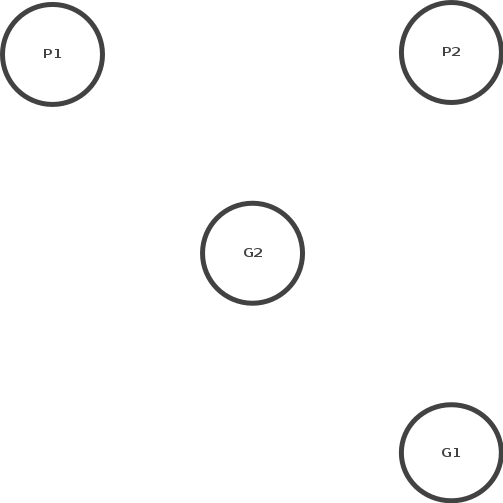
\includegraphics[width=0.5\textwidth]{img/descripcion/descripcion_ejemplo_entrada.png}
		\caption{Mapa de entrada ejemplo.}
		\label{fig: descripcion_ejemplo_entrada}
	\end{center}
\end{figure}

\par En la figura \ref{fig: descripcion_ejemplo_entrada} podemos ver un mapa que corresponde a un ejemplo de datos de entrada del problema. Veamos en detalle este ejemplo. Tenemos una mochila con capacidad 5 y dos nodos P y dos nodos G con las siguientes características:

\begin{itemize}
	\item $P_1$: nodo P ubicado en (2, 1).
	\item $P_2$: nodo P ubicado en (2, 3).
	\item $G_2$: nodo G ubicado en (4, 3) y con cantidad de pociones necesarias igual a 3.
	\item $G_2$: nodo G ubicado en (3, 2) y con cantidad de pociones necesarias igual a 2.
\end{itemize}

\par Para este caso en particular, el camino mas corto es el que se muestra en la figura \ref{fig: descripcion_ejemplo_solucion}. Podemos ver que el camino comienza en el nodo $P_1$ donde obtiene 3 pociones, va hacia el nodo $G_2$, donde pierde 3 pociones y queda sin ninguna; luego hacia el nodo $P_2$, donde obtiene 3 pociones; y finaliza en el nodo $G_1$, perdiendo 2 pociones y quedando sólo con una. En la figura vemos también que están detalladas las distancias entre los nodos del camino. Finalmente, este camino nos da una distancia total de 4.82842 y es una solución al problema.

\begin{figure}[h]
	\begin{center}
		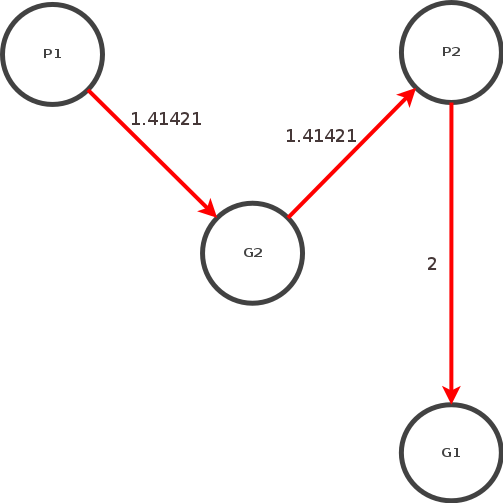
\includegraphics[width=0.4\textwidth]{img/descripcion/descripcion_ejemplo_solucion.png}
		\caption{Mapa de entrada ejemplo con el camino solución marcado.}
		\label{fig: descripcion_ejemplo_solucion}
	\end{center}
\end{figure}

\par En este informe se van a presentar distintos tipos de algoritmos para resolver este problema. En primer lugar, un algoritmo exacto. Luego, algoritmos basados en heurísticas y metaheurísticas. Se compararán los distintos algoritmos para determinar cuál responde mejor al problema planteado en función de tiempos y precisión de la solución.

\newpage

\section{Ejercicio 1: Algoritmo exacto}
\subsection{Introducción y descripción del algoritmo}

\par Para un primer acercamiento a la solución, buscaremos resolver el problema mediante un algoritmo exacto, es decir, un algoritmo que nos de la solución exacta al problema y no un acercamiento (como veremos mas adelante). En este caso, como no encontramos algoritmos polinomiales que nos brinden la solución al problema, diseñamos un algorítmo de fuerza bruta (backtraking) para ver cómo se comporta y tener un valor exacto de la solución que nos sirva para comparar otros tipos de algoritmos.

\par Un algoritmo de fuerza bruta (o backtraking) se basa en recorrer todas los posibles caminos a la solución hasta encontrarla. El problema en cuestión se trata de encontrar el camino mínimo entre nodos que cumpla ciertas condiciones, por lo que nuestro algoritmo de fuerza bruta recorrerá los nodos de todas las formas válidas (que se cumplan las condiciones pedidas) posibles. A medida que hace esto, irá guardando el mínimo camino conseguido hasta el momento. Cuando finalice todos los caminos posibles podrá asegurar que el camino guardado es el mínimo, ya que recorrió todas las posibles instancias del problema y comparó todos los caminos válidos.

\par Se ve que es un algoritmo simple, se basa en recorrer todas las posibilidades y quedarse con la mejor. El problema se da en que recorrer todas las instancias de un problema suele ser muy pesado. Para algunos problemas, este algoritmo puede ser una herramienta, pero en general, con problemas relativamente grandes (o mejor dicho, no muy acotados), lleva mucho tiempo de computo. Veremos mas adelante que su complejidad aumenta fuértemente en base a algunos parámetros, y esto lo hace muy difícil de correr.

\subsection{Idea general del algoritmo}

\par Previamante contamos que había dos tipos de nodos: gimnasios y paradas. Un jugador puede ir de un nodo a cualquier otro que no haya visitado antes. Por lo que solo nos manejaremos con nodos restantes (los que el jugador aún no visitó) y nodos en el camino (los que sí fueron visitados), y no con enlaces entre ellos (lo que habitualmente se hace cuando se trata de grafos). Entre dos nodos cualesquiera existe una distancia, que calcuaremos al inicio. También es importante notar que para ir a un nodo de tipo gimnasio se debe contar con una serie de pociones. Pero al comenzar el jugador no cuenta con ninguna, por lo que el primer nodo ha visitar siempre debe ser uno del tipo parada.

\par Aclarados estos detalles, retomaremos el ejemplo mostrado en la descripción general del problema (figura \ref{fig: descripcion_ejemplo_entrada}), veremos las distancias entre estos nodos y analizaremos el funcionamiento del algoritmo sobre este caso en particular.

\begin{table}[h]
	\centering
	\begin{tabular}{|>{\centering\arraybackslash}p{2cm}|>{\centering\arraybackslash}p{2cm}|>{\centering\arraybackslash}p{2cm}|>{\centering\arraybackslash}p{2cm}|>{\centering\arraybackslash}p{2cm}|}
		\hline
		   & \textbf{G1} & \textbf{G2} & \textbf{P1} & \textbf{P2} \\ \hline
		\textbf{G1} & \cellcolor{gray} & 1.41421 & 2.82842 & 2 \\ \hline
		\textbf{G2} & 1.41421 & \cellcolor{gray} & 1.41421 & 1.41421 \\ \hline
		\textbf{P1} & 2.82842 & 1.41421 & \cellcolor{gray} & 2 \\ \hline
		\textbf{P2} & 2 & 1.41421 & 2 & \cellcolor{gray} \\
		\hline
	\end{tabular}
	\caption{Distancias entre los nodos del caso de ejemplo.}
	\label{fig: ejercicio1_ejemplo_distancias}
\end{table}

\par En la figura \ref{fig: ejercicio1_ejemplo_distancias} podemos ver las distancias entre los distintos nodos. Vale aclarar que no importa la dirección en la que vaya el jugador, sino los nodos entre los cuales se mueve. Por ejemplo, ir de \textit{P1} a \textit{P2} cuesta 2, igual que ir de \textit{P2} a \textit{P2}.

\par Como comentamos en la introducción, el algoritmo se basa en recorrer los caminos válidos y quedarse con el mejor (mínima distancia). Por lo tanto, al tomar este ejemplo de entrada, el algoritmo comenzará parándose sobre un nodo \textit{i} del tipo parada y calculará todos los caminos posibles partiendo desde él. Luego hará lo mismo para cada uno de los nodos restantes del tipo parada. En el ejemplo, si comienza por el nodo \textit{P1} podrá alcanzar los caminos que se observan en la figura \ref{fig: ejercicio1_ejemplo_caminos1}. En verde están marcadas las distancias mínimas, porque nosotros ya conocemos la solución, pero el algoritmo las toma como mínimo parcial y no sabe aún si van a ser los mínimos generales. Esto porque todavía le quedan por ver todos los caminos que comienzan en el nodo P2.

\begin{figure}[H]
    \begin{subfigure}[b]{0.49\textwidth}
        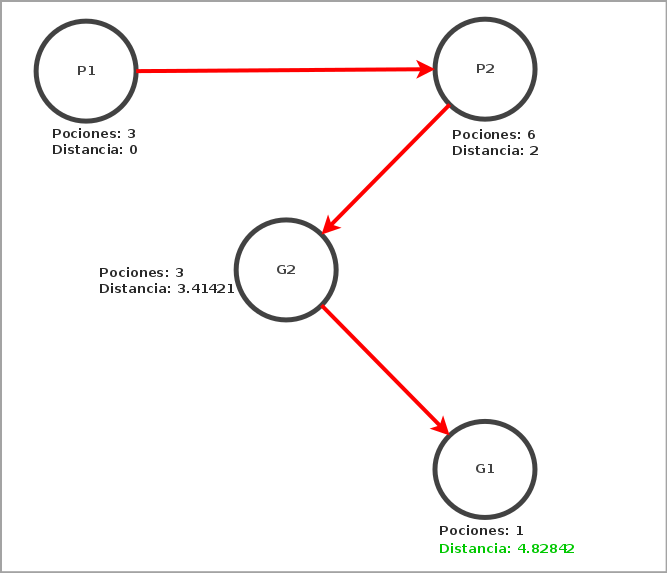
\includegraphics[width=\linewidth]{img/ejercicio1/ejercicio1_ejemplo_camino1_1.png}
        \caption{Camino válido y solución.}
        \label{fig: ejercicio1_ejemplo_camino1_1}
    \end{subfigure}
    \begin{subfigure}[b]{0.49\textwidth}
        \includegraphics[width=\linewidth]{img/ejercicio1/ejercicio1_ejemplo_camino1_2.png}
        \caption{Camino válido y solución.}
        \label{fig: ejercicio1_ejemplo_camino1_2}
    \end{subfigure}
    \begin{subfigure}[b]{0.49\textwidth}
        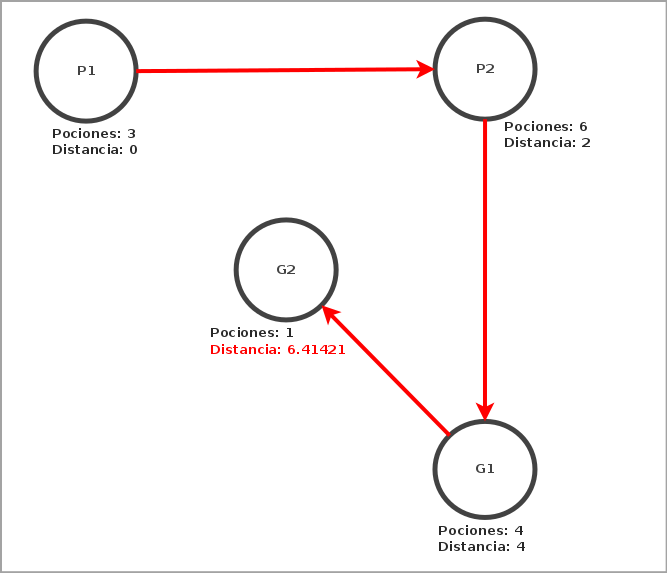
\includegraphics[width=\linewidth]{img/ejercicio1/ejercicio1_ejemplo_camino1_3.png}
        \caption{Camino válido.}
        \label{fig: ejercicio1_ejemplo_camino1_3}
    \end{subfigure}
    \begin{subfigure}[b]{0.49\textwidth}
        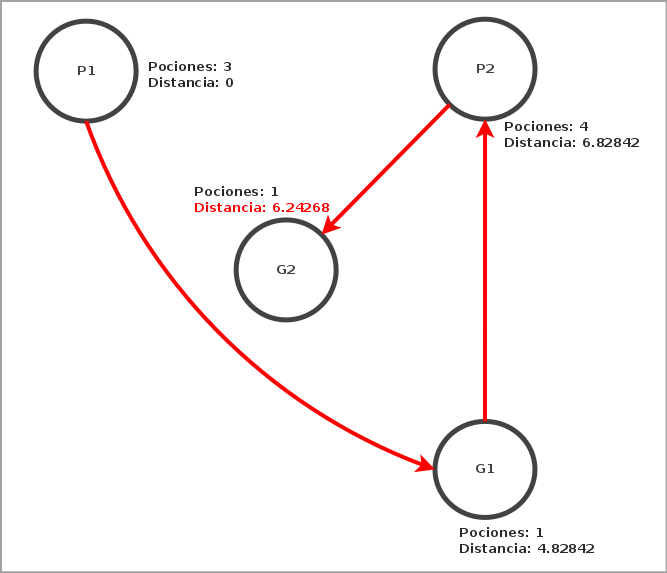
\includegraphics[width=\linewidth]{img/ejercicio1/ejercicio1_ejemplo_camino1_4.png}
        \caption{Camino válido.}
        \label{fig: ejercicio1_ejemplo_camino1_4}
    \end{subfigure}
    \caption{Caminos válidos alcanzados por el algoritmo partiendo del nodo P1. En verde se marcan las distancias mínimas.}
    \label{fig: ejercicio1_ejemplo_caminos1}
\end{figure}

\par El algoritmo, procede a tomar el nodo P2 y calcular todos los caminos que comienzan en él. En la figura \ref{fig: ejercicio1_ejemplo_caminos2} podemos ver todos los caminos válidos que parten del nodo P2. Luego, puede determinar que la distancia mínima es \textbf{4.82842}, y puede tomar como solución cualquiera de los caminos que verificó que dan este resultado.

\begin{figure}[H]
    \begin{subfigure}[b]{0.49\textwidth}
        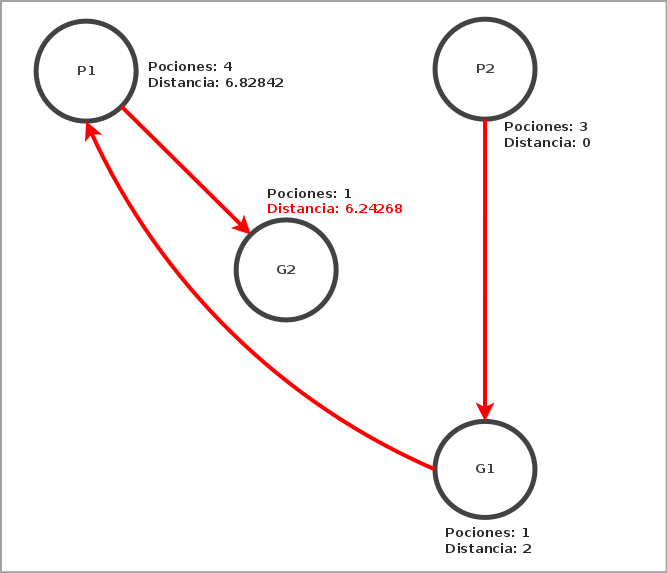
\includegraphics[width=\linewidth]{img/ejercicio1/ejercicio1_ejemplo_camino2_1.png}
        \caption{Camino válido.}
        \label{fig: ejercicio1_ejemplo_camino2_1}
    \end{subfigure}
    \begin{subfigure}[b]{0.49\textwidth}
        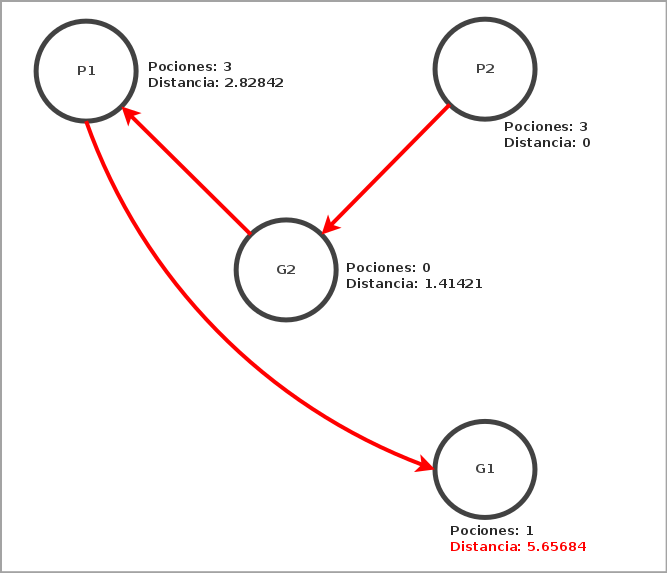
\includegraphics[width=\linewidth]{img/ejercicio1/ejercicio1_ejemplo_camino2_2.png}
        \caption{Camino válido.}
        \label{fig: ejercicio1_ejemplo_camino2_2}
    \end{subfigure}
    \begin{subfigure}[b]{0.49\textwidth}
        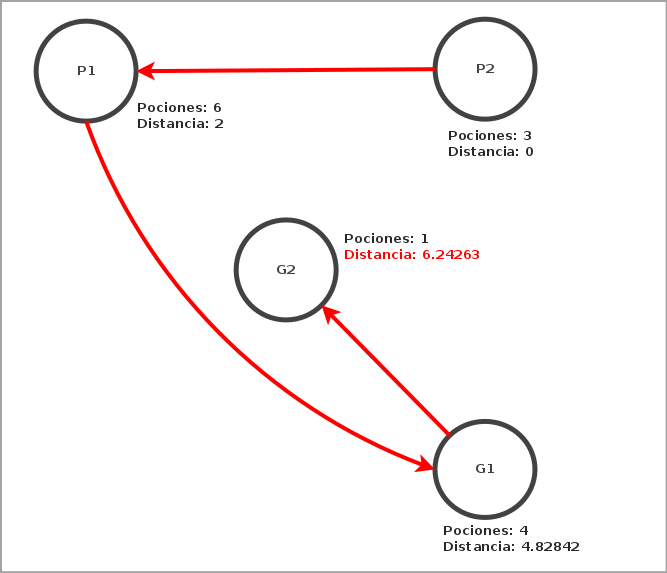
\includegraphics[width=\linewidth]{img/ejercicio1/ejercicio1_ejemplo_camino2_3.png}
        \caption{Camino válido.}
        \label{fig: ejercicio1_ejemplo_camino2_3}
    \end{subfigure}
    \begin{subfigure}[b]{0.49\textwidth}
        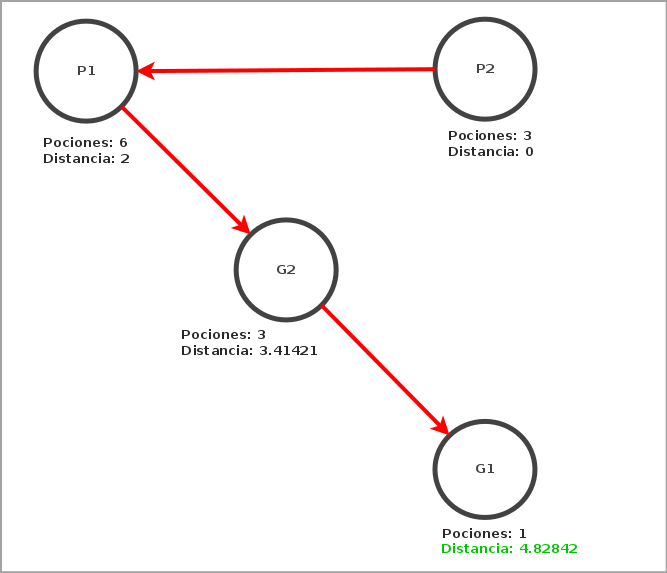
\includegraphics[width=\linewidth]{img/ejercicio1/ejercicio1_ejemplo_camino2_4.png}
        \caption{Camino válido y solución.}
        \label{fig: ejercicio1_ejemplo_camino2_4}
    \end{subfigure}
    \caption{Caminos válidos alcanzados por el algoritmo partiendo del nodo P1. En verde se marcan las distancias mínimas.}
    \label{fig: ejercicio1_ejemplo_caminos2}
\end{figure}

\par Si miramos en detalle las figuras \ref{fig: ejercicio1_ejemplo_camino1_1} y \ref{fig: ejercicio1_ejemplo_camino2_4} podemos ver que ambos caminos llegan al nodo G2 con 3 pociones y solo tienen como no visitado el nodo G1. Por lo que si nos paramos en ese instante, el subproblema pasa a ser saber el camino mínimo partiendo del nodo G2 con 3 pociones y teniendo como nodos a G2 y G1. Luego de definir este subproblema podemos notar que en ambos casos se resuelve de la misma manera este subproblema. En un caso de tamaño muy acotado, como este ejemplo, calcular dos veces un subproblema puede no ser relevante, pero para casos más grandes estos subproblemas repetidos pueden crecer expoencialmente. Para evitar calcular más de una vez un mismo subproblema vamos a definir las instancias: una instancia consta de un nodo en el cual el jugador está parado, una cantidad de pociones que tiene en su mochila y una serie de nodos habilitados para visitar. Una vez calculada una instancia será guardada, lo que nos asegura que al darse otra vez este subproblema podemos recurrir a este valor precalculado y evitar tiempo de procesamiento. más adelante expererimentaremos sobre un algoritmo básico que no tiene en cuenta las instancias y otros que si guardan las instancias (y adoptan otras mejoras) y veremos las diferencias para casos un poco más grandes.

\subsection{Explicación del algoritmo}

\par Para nuestro algoritmo de fuerza bruta utilizamos una función recursiva que se encargue de calcular una instancia. Va a tomar como parámetros:

\begin{itemize}
	\item \textbf{nodo actual:} para identificar la instancia,
	\item \textbf{nodos de tipo parada restantes:} para identificar la instancia,
	\item \textbf{nodos de tipo gimnasio restantes:} para identificar la instancia,
	\item \textbf{pociones en la mochila:} para identificar la instancia,
	\item \textbf{camino recorrida hasta el momento:} para saber si se alcanzó un nuevo camino mínimo o no (sumando la distancia recorrida más el subcamino mínimo calculado en la instancia).
\end{itemize}

\par La función va a llamarse recursivamente para todas las instancias que se desprendan de ella. Por ejemplo, si estamos en un nodo A y podemos pasar al nodo B la función se llamará recursivamente con B como nodo actual, el camino agregando a B al final, actualizando la cantidad de pociones (según corresponda) y quitando a B de los nodos restantes. Veamos un pseudocódigo para entender mejor el funcionamiento.

\par En el pseudocódigo \ref{algo: ejercicio1_pseudocodigo} podemos observar el algoritmo de la función que calcula el camino mínimo dada una instancia del problema. Analicemos su funcionamiento:

\begin{itemize}
	\item Lo primero que se hace es verificar si la instancia ya fué calculada. En ese caso, no se vuelve a calcular y se avanza a devolver esa solución.
	\item Luego se inicializa $solucion$ como inválida. En esta variable se va a guardar la solución (camino mínimo) parcial de la instancia.
	\item Se verifica que queden nodos del tipo gimnasio por recorrer. Recordemos que no es una condición necesaria pasar por todos los nodos de tipo parada, y si se siguiera recorriendo se obtendría un camino mayor, que no sería solución. Si no quedan gimnasios se devuelve un camino con tan solo en nodo actual y distancia 0.
	\item En la linea 8 y 9 se ordenan las listas de nodos restantes por distancia al nodo actual. Esto es una estragia para intentar visitar primero los nodos más cercanos y así lograr alcanzar el camino mínimo más rápido.
	\item Luego se llama recursivamente a la función para cada nodo que pueda ser visitado y se verifica cuál de las soluciones devueltas resulta ser el mínimo de la instancia.
\end{itemize}

\medskip

\SetAlgoLined
\SetKwProg{Fn}{Function}{:}{EndFunction}
\begin{algorithm}[H]
	\label{algo: ejercicio1_pseudocodigo}
	\Fn{calcular\_instancia(camino\_actual: lista(nodo), paradas\_a\_recorrer: lista(nodo), gimnasios\_a\_recorrer: lista(nodo), pociones: int)}{
		\BlankLine
		
		\If{la instancia no fué calculada aún}{
			\BlankLine
			
			$nodo\_actual \gets camino\_actual[|camino\_actual|-1]$\\
			$solucion \gets \O$

			\BlankLine
			\uIf{$| gimnasios\_a\_recorrer | = 0$}{
				\BlankLine
				
				$solucion \gets $camino formado solo por $nodo\_actual$
				
				\BlankLine
			}
			\uElse{
				\BlankLine
				
				ordena $gimnasios\_a\_recorrer$ por distancia a $nodo\_actual$ (de menor a mayor)
				ordena $paradas\_a\_recorrer$ por distancia a $nodo\_actual$ (de menor a mayor)

				\BlankLine
				\For{nodo\_vecino en $gimnasios\_a\_recorrer$}{
					
					\BlankLine
					\If{$pociones \geq pocionesNecesarias(nodo\_vecino)$}{
						\BlankLine

						$subsolucion \gets calcular\_instancia(camino\_actual + nodo\_vecino, paradas\_a\_recorrer, gimnasios\_a\_recorrer - nodo\_vecino, pociones - pocionesNecesarias(nodo\_vecino))$

						\BlankLine
						\uIf{$esValida(subsolucion) \wedge ( \neg esValida(solucion) \vee distancia(subsolucion + nodo\_actual) \leq distancia(solucion) )$}{
							\BlankLine
						
							$solucion \gets subsolucion + nodo\_actual$
						
							\BlankLine
						}
					}
				}

				\BlankLine
				\If{$pociones < mochila$}{
					\BlankLine

					\For{nodo\_vecino en $paradas\_a\_recorrer$}{
						\BlankLine

						$subsolucion \gets calcular\_instancia(camino\_actual + nodo\_vecino, paradas\_a\_recorrer - nodo\_vecino, gimnasios\_a\_recorrer, pociones + 3)$

						\BlankLine
						\uIf{$esValida(subsolucion) \wedge ( \neg esValida(solucion) \vee distancia(subsolucion + nodo\_actual) \leq distancia(solucion) )$}{
							\BlankLine
						
							$solucion \gets subsolucion + nodo\_actual$
						
							\BlankLine
						}
					}
				}
			}
			\BlankLine

			$instancia\_actual \gets solucion$
			\BlankLine
		}
		\BlankLine
		
		\Return $instancia\_actual$
		
		\BlankLine
	}
	\caption{Función encargada de calcular el valor asignado al exponente pasado como parámetro, según el número pasado por parámetro.}
\end{algorithm}



\subsection{Podas y Estrategias}

\par Al tratarse de una algoritmo de fuerza bruta, los tiempos de ejecución suelen ser muy grandes. Por esto, suelen adoptarse estrategias para tratar de disminuirlos. A continuación vamos a explicar las distintas estrategias y podas que se implementaron para este problema.

\par En primer lugar, el diseño del algoritmo se basa fuértemenete en las \textit{instancias} antes mencionadas. La idea es que si ya se calculó una instancia, no vuelva a calcularse. A partir de esto, se podan una enorme cantidad de ramas de cálculo. El problema que surje a partir de esto es que las instancias dependen de los nodos restantes, y no del camino recorrido. Por ende, el hecho de contar con una cota de camino mínimo no te permite podar el cálculo de una instancia. Por ejemplo, supongamos que tenemos 5 nodos: \textit{A, B, C, D, E}. Si debemos calcular la instancia donde el nodo actual es C y los nodos restantes son D y E (sin tener en cuenta las pociones ni los tipos de nodo), no podemos diferenciar si el camino para llegar a C fue A,B o B,A. Por esto, no podemos cortar el cálculo de la instancia por la distancia del camino previo, ya que si se llega a la misma instancia con otro camino previo el resultado puede ser mejor, o hasta incluso la solución del problema. Esto nos limita bastante a la hora de implementar podas que disminuyan los tiempos de ejecución.

\par En cuanto a estrategias tomadas, podemos mencionar:

\begin{itemize}
	\item chequear que la distancia a un nodo al que vamos a ir sea menor que la distancia mínima calculada hasta el momento. De esta manera podemos asegurar que no hay ninguna forma de que nos sirva ir a ese nodo en busca del camino mínimo.
	\item al igual que el caso anterior, pero con el camino mínimo global calculado hasta el momento.
	\item ordenar los gimnasios por la distancia al nodo actual, de menor a mayor. La idea de esta estrategia es que nos conviene ir a los nodos que tenemos más cerca. Es una idea basada en un algoritmo goloso, tratar de ir primero a lo más cercano, y así conseguir un camino menor.
	\item al igual que el caso anterior, pero con los nodos de tipo parada.
	\item visitar primero los nodos del tipo gimnasio. Esta es otra idea basada en un algoritmo goloso, ya que uno quiere visitar todos los nodos del tipo gimnasio en la menor distancia. Entonces se intenta ir primero a nodos de tipo gimnasio.
	\item no recorrer más nodos si ya se han recorrido todos los del tipo gimnasio. El problema pide recorrer todos los gimnasios, pero no es necesario recorrer el resto. Por esto, una vez que se han recorrido todos los gimnasios no se continúa.
	\item si la mochila del jugador se encuentra llena, no se recorren más paradas. Si no hay capacidad para guardar más pociones, no sirve de nada visitar más nodos del tipo parada, ya que eso implicaría más distancia (por la desigualdad triangular).
	\item se realiza un goloso para tener una cota inicial. De esta manera, se tiene un camino mínimo parcial para ser utilizado como cota.
\end{itemize}

\par más adelante, en la sección de Experimentación (Sección \ref{subsec: ejercicio1_experimentacion}), se analizarán las distintas estrategias y podas y se verá su comportamiento con distintos tipos de entrada en función del tiempo de ejecución y otras variables.



\subsection{Análisis de complejidad}

\par Para analizar la complejidad del algoritmo y su implementación debemos definir ciertos conceptos y parámetros:

\begin{itemize}
	\item \textbf{n}: Cantidad de nodos del tipo gimnasio.
	\item \textbf{m}: Cantidad de nodos del tipo parada.
	\item \textbf{k}: Capacidad de la mochila del jugador.
\end{itemize}

\par A continuación vamos a ver las partes importantes y relevantes del algoritmo y analizaremos la complejidad. Primero, veamos la función $calcular\_instancia$.

\begin{itemize}
	\item Calcular el número de instancia es O($n+m$). Esto porque se arma un número binario con la posición $N_i$=1 si el nodo $i$ está en la instancia o $N_i$=0 si no y luego se pasa de binario a decimal. Es importante tener en cuenta también que se deben calcular potencias de 2.
	\item Ordenar los nodos de tipo parada cuesta O($m^2$).
	\item Ordenar los nodos de tipo gimnasio cuesta O($n^2$).
	\item Tanto calcular la distancia como copiar el vector $gimnasios\_a\_recorrer$ cuesta O($n$) y se realiza para cada nodo en el vector $gimnasios\_a\_recorrer$. Entonces nos queda O($n^2$).
	\item Calcular la distancia cuesta y copiar el vector $paradas\_a\_recorrer$ cuesta O($n+m$) y se realiza para cada nodo en el vector $paradas\_a\_recorrer$. Entonces nos queda O($m \cdot (n+m)$).
	\item En total, tenemos que la función $calcular\_instancia$ cuesta O($n+m + m^2 + n^2 + m^2 + m \cdot (n+m)$) = O($n^2 + m^2 + n \cdot m$) = \textbf{O($\boldsymbol{n^2 + m^2}$)}.
\end{itemize}

\par Tenemos entonces que la función $calcular\_instancia$ cuesta O($n^2 + m^2$). Recordemos que esta función se utilizaba para para calcular una instancia, y nunca calcula dos veces la misma instancia. Veamos entonces la cantidad màxima de instancias. Una instancia se diferenciaba por:

\begin{itemize}
	\item \textbf{nodo actual}: la cantidad máxima de nodos es $n+m$.
	\item \textbf{pociones}: la cantidad máxima de pociones està acotada por la capacidad de la mochila: $k$.
	\item \textbf{nodos restantes}: el número binario de instancia tiene longitud $n+m$ (una posición por cada nodo). Al pasarlo a entero, tenemos $2^{n+m}$. Porque el número máximo sería el que tiene todas las posiciones en 1: $\sum_{i=0}^{n+m-1}2^i$ = $2^{n+m}-1$. Tengamos en cuenta que iniciamos a contar en 0. Entonces de 0 a $2^{n+m}-1$ tenemos $2^{n+m}$ números.
\end{itemize}

\par De esta manera vemos que tenemos $(n+m) \cdot k \cdot 2^{n+m}$ posibles instancias. En general, se calcularán muchas menos instancias, pero existen casos donde se calcula esa cantidad, por lo que es una cota superior.

\par Tenemos entonces que la función $calcular\_instancia$ cuesta O($n^2 + m^2$) y puede llegar a ejecutarse $(n+m) \cdot k \cdot 2^{n+m}$ veces. Por lo tanto esta implementación tiene una complejidad O($(n^2 + m^2) \cdot (n+m) \cdot k \cdot 2^{n+m}$). Veamos mejor la primera parte de esta cota: $n^2 + m^2 \cdot (n+m)$.

\begin{equation}
	(n^2 + m^2) \cdot (n+m) = n^3 + n^2 \cdot m + m^3 + m^2 \cdot n
\end{equation}

Si $n > m$, tenemos que O($n^3 + n^2 \cdot m + m^3 + m^2 \cdot n$) = O($n^3$). Si en cambio $m > n$, tenemos que O($n^3 + n^2 \cdot m + m^3 + m^2 \cdot n$) = O($m^3$). Si en cambio, $n = m = l$, tenemos que O($n^3 + n^2 \cdot m + m^3 + m^2 \cdot n$) = O($l^3$). Por esto, podemos decir que O($n^3 + n^2 \cdot m + m^3 + m^2 \cdot n$) = O($n^3 + m^3$). Entonces volviendo a la complejidad del problema nos queda \textbf{O($\boldsymbol{(n^3 + m^3) \cdot k \cdot 2^{n+m}}$)}.



\subsection{Experimentación}
\label{subsec: ejercicio1_experimentacion}

\par Antes de comenzar la experimentación, vamos a definir las distintas versiones del programa:

\begin{itemize}
	\item \textbf{Versión 0}:
		\begin{itemize}
			\item No almacena las instancias calculadas, por lo cual puede calcular más de una vez el mismo subcamino.
			\item Intenta ir siempre primero a los gimnasios.
			\item No va a una parada si no tiene capacidad para almacenar nuevas pociones.
			\item No va a más paradas si no quedan gimnasios por recorrer.
		\end{itemize}
	\item \textbf{Versión 1}:
		\begin{itemize}
			\item Incluye todas las estrategias y podas de la versión 0.
			\item Almacena las instancias calculadas.
		\end{itemize}
	\item \textbf{Versión 2}:
		\begin{itemize}
			\item Incluye todas las estrategias y podas de la versión 1.
			\item Verifica que la distnacia al siguiente nodo (al cual va a moverse) no supere la distancia mínima parcial (de su misma instancia).
			\item Verifica que la distnacia al siguiente nodo (al cual va a moverse) no supere la distancia mínima parcial global (de todas las instancias).
		\end{itemize}
	\item \textbf{Versión 3}:
		\begin{itemize}
			\item Incluye todas las estrategias y podas de la versión 2.
			\item En cada instancia, ordena los gimnasios según la distancia al nodo actual (de menor a mayor). Con esto intenta ir primero a los gimnasios más cercanos.
			\item En cada instancia, ordena las paradas según la distancia al nodo actual (de menor a mayor). Con esto intenta ir primero a las paradas más cercanas.
		\end{itemize}
	\item \textbf{Versión 4}:
		\begin{itemize}
			\item Incluye todas las estrategias y podas de la versión 3.
			\item Al comenzar la ejecución, corre una heurística golosa. Conserva este resultado como cota superior.
		\end{itemize}
\end{itemize}

\par La versión 0 nos servirá de guía para ver cuánto influye el almacenamiento de instancias en los tiempos de ejecución. Luego veremos en cada versión cuanto influye la incorporación de cada poda y estrategia en los tiempos de ejecución.

\par A continuación se correrán distintos casos con ciertas características para ver el comportamiento de las distintas versiones del programa.

\subsubsection{Experimento 1: Cantidad de paradas vs Tiempos de ejecución}

\par En el primer experimento vamos a analizar los tiempos de ejecución en función de la cantidad de paradas. Para esto, vamos a dejar fija la cantidad de gimnasios y la capacidad de la mochila, iremos aumentando la cantidad de paradas y veremos cómo se comportan los tiempos de ejecución.

\par Tomaremos \textit{cantidad de gimnasios = 3} y \textit{capacidad de la mochila = 5}. Vamos a comenzar con \textit{cantidad de paradas = 1} y la iremos aumentando hasta llegar a 15. Generaremos los casos de entrada de forma aleatoria, respetando los parámetros y verificando que tengan solución.

\par Esperamos ver una gran diferencia entre la Versión 0 y las restante, ya que va a calcular muchas instanncias repetidas veces y el resto no. Entre las otras, no esperamos ver gran diferencia, pero nos gustaría que con mas estrategias y podas mejoren los tiempos.

\begin{figure}[H]
	\begin{center}
		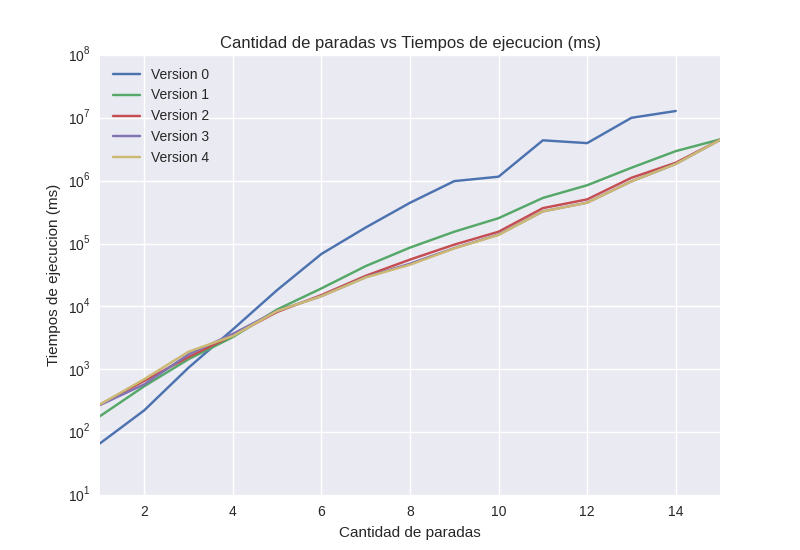
\includegraphics[width=\textwidth]{img/ejercicio1/exp1_1.png}
		\caption{Resultados del experimento 1.}
		\label{fig: ej1_exp1_1}
	\end{center}
\end{figure}

\par En la figura \ref{fig: ej1_exp1_1} podemos ver los resultados del experimento 1. Como esperábamos, la versión 0 cuenta con los tiempos más altos y supera al resto ampliamente (teniendo en cuenta que el gráfico se muestra con escala logarítima). En un comienzo, la versión 0 toma menos tiempo de procesamiento, porque los casos de entrada son muy pequeños e influye mucha inicializar la estructura de instancias. Pero a partir de 4 paradas se ve como se desprende del resto y se eleva con mucha más rapidez.

\par Para poder ver mejor los resultados de las versiones 1, 2, 3 y 4, en la figura \ref{fig: ej1_exp1_2} se excluyó a la versión 0 y se centró el foco en las cantidad de paradas mayores a 8. Podemos ver que no se toman grandes diferencias. También es interesante que entre la versión 3 y la 4 no se sacan diferencias. Creemos que esto se debe a que a partir de una cierta cantidad de paraadas el cálculo de la herística golosa deja de influir. Podemos decir entonces que en cuanto a la cantidad de paredes, nos conviene quedarnos con la versión 3 ó 4.

\begin{figure}[H]
	\begin{center}
		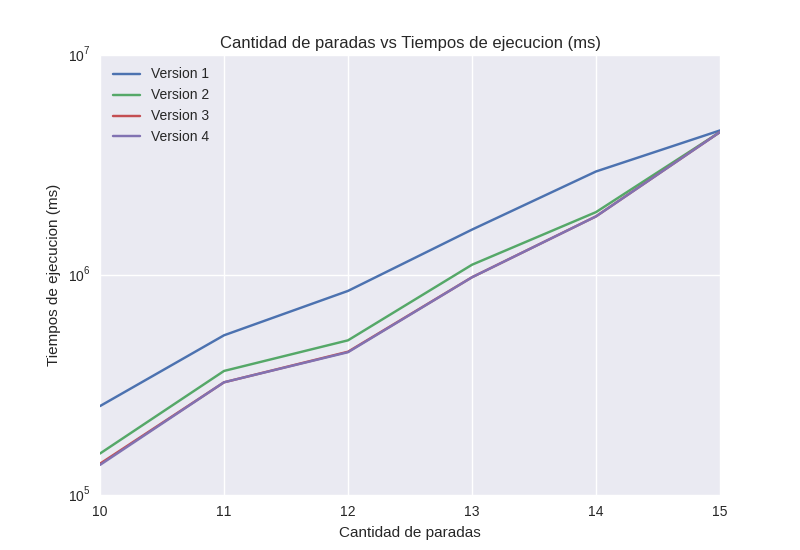
\includegraphics[width=\textwidth]{img/ejercicio1/exp1_2.png}
		\caption{Resultados del experimento 1 ampliado en las cantidades de paradas mayores a 8 y excluyendo la versión 0.}
		\label{fig: ej1_exp1_2}
	\end{center}
\end{figure}


\subsubsection{Experimento 2: Cantidad de gimnasios vs Tiempos de ejecución}

\par En este experimento vamos a analizar los tiempos de ejecución en función a la cantidad de gimnasios. Vamos a fijar los parámetros \textit{cantidad de paredes} y \textit{capcidad de la mochila} y veremos como se comportan las distintas versiones del programa.

\par Tomaremos \textit{cantidad de paredes = 4} y \textit{capacida de la mochila = 4}. Iremos aumentando \textit{cantidad de gimnasios} desde 1 hasta 10 y generaremos una serie de casos aleatorios respetando los parámetros. Los casos de entrada se generan de forma tal que siempre exista solución al problema.

\par Esperamos nuevamente que la versión 0 se encuentre lejana al resto. No creemos que las otras versiones se distancien mucho entre sí, ya que todas intentan primero ir a un gimnasio, por lo que no van a podar mucho estos caminos.

\begin{figure}[H]
	\begin{center}
		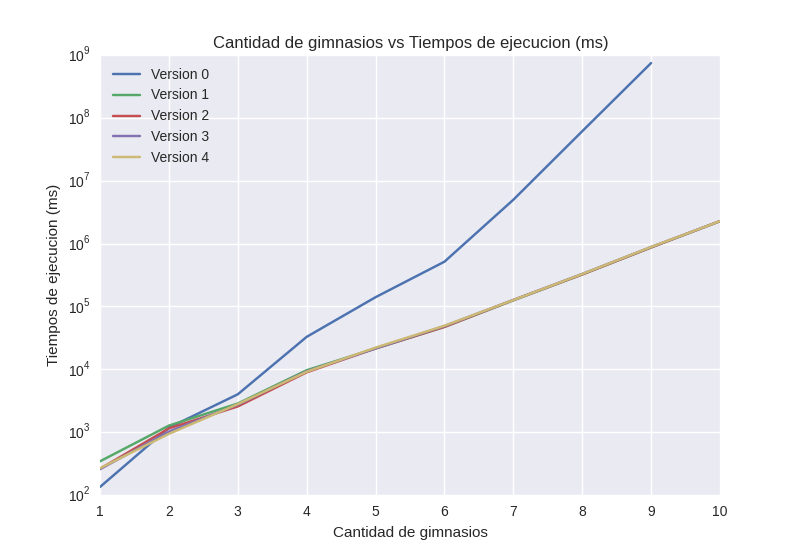
\includegraphics[width=\textwidth]{img/ejercicio1/exp2_1.png}
		\caption{Resultados del experimento 2.}
		\label{fig: ej1_exp2_1}
	\end{center}
\end{figure}

\par Podemos ver en la figura \ref{fig: ej1_exp2_1} los resultados del experimento. Vemos que se cumple lo que esperábamos sobre la versión 0 y notamos que las versiones 1, 2, 3 y 4 se encuentran casi superpuestas.




\subsubsection{Experimento 3: Capacidad de la mochila vs Tiempos de ejecución}

\par En este experimento vamos a variar la capacidad de la mochila y analizar el comportamiento de las versiones del programa. Dejaremos fijos los parámetros \textit{cantidad de paradas} y \textit{cantidad de gimnasios} y analizaremos los tiempos de ejecución de cada versión en base al parámetro \textit{capacidad de la mochila}.

\par Aquí también se espera que la versión 0 tenga tiempos de ejecución mayores al resto. Viendo los resultados de los experimentos previos, no esperamos grandes diferencias entre los restantes, ya que la condición a la que afecta la capacidad de la mochila es si puedo ir a un gimnasio o no, y esta condición afecta a todas las versiones por igual.

\par Para llevar a cabo el epxerimento vamos a tomar \textit{cantidad de gimnasios = 4} y \textit{cantidad de paradas = 4} e iremos aumentando el parámetro \textit{capacidad de la mochila} desde 1 hasta 10. Los casos de entrada serán generados de la misma forma que los dos experimentos previos.

\begin{figure}[H]
	\begin{center}
		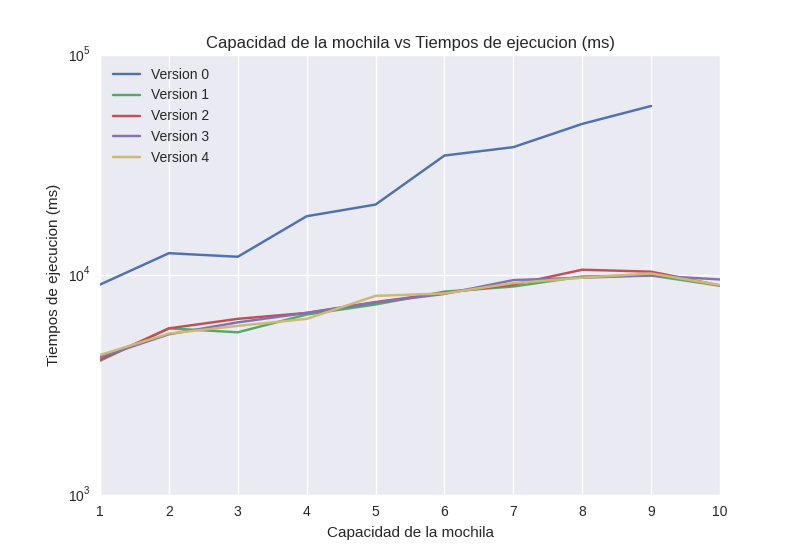
\includegraphics[width=\textwidth]{img/ejercicio1/exp3_1.png}
		\caption{Resultados del experimento 3.}
		\label{fig: ej1_exp3_1}
	\end{center}
\end{figure}

\par En la figura \ref{fig: ej1_exp3_1} podemos ver los resultados del experimento 3. Podemos ver que las podas hacen que las versiones 1, 2, 3 y 4 mejores mucho los tiempos de ejecución. Pero también notamos que no se observan grandes diferencias entre ellas. Ninguna versión se acomoda por debajo del resto en cuanto a tiempos de ejecución.

\par Ninguno de los 3 experimentos nos dio un resultado desfavorable para la versión 4. Por lo que creemos que lo mejor es utilizar esta versión que incluye una cota de heurística golosa y no parece ser influyente en los tiempos de ejecución.


\subsubsection{Experimento 4: Pociones necesarias para los gimnasios - TSP vs no-TSP}

\par Hasta el momento siempre tomamos casos donde el jugador necesitaba pociones para ir a los gimnasios. Pero un caso particular es cuando no necesita pociones para ir a ningún gimnasio, por lo cual no necesita visitar paradas. En este caso, el problema termina siendo calcular la distancia mínima que se debe recorrer para visitar todos los nodos del tipo gimnasio. Este problema es conocido como `El problema del viajante de comercio' (TSP: Traveling Salesman Problem).

\par En este experimento, vamos a tratar ese caso particular. Por lo que vamos a variar el parámetro $Pociones necesarias para un gimnasio$ entre 0 y 3. El caso en que valga 0 va a ser el caso de TSP. Queremos ver como se comporta el algoritmo para este caso particular y determinar si se trata de un mejor o peor caso o si no se diferencia del resto. Por el diseño del algoritmo, siempre se comienza por un nodo del tipo parada. Por lo que siempre vamos a dejar un nodo del tipo parada (aunque se trate de un TSP y solo se necesiten gimnasios).

\par Para esto vamos a fijar el parámetro $Capacidad de la mochila$ y vamos a comenzar con 2 nodos e iremos aumentando esta cantidad de a 2. Dependiendo si se trata de el caso TSP o no tomaremos distintas determinaciones:

\begin{itemize}
	\item \textbf{TSP}: siempre habrá un nodo de tipo parada y el resto de tipo gimnasio.
	\item \textbf{no-TSP}: tomaremos $Cantidad de paradas = Cantidad de gimnasios = \frac{nodos}{2}$.
\end{itemize}

\par Para cada caso, generamos los nodos (y sus ubicaciones) y se le aplicó un valor distinto al parámetro $Pociones necesarias para un gimnasio$ dependiendo el caso. Inclusive, se modificó la cantidad de paradas o gimnasios. Pero no así las ubicaciones, por lo que siempre se utilizan los mismos nodos.

\begin{figure}[H]
	\begin{center}
		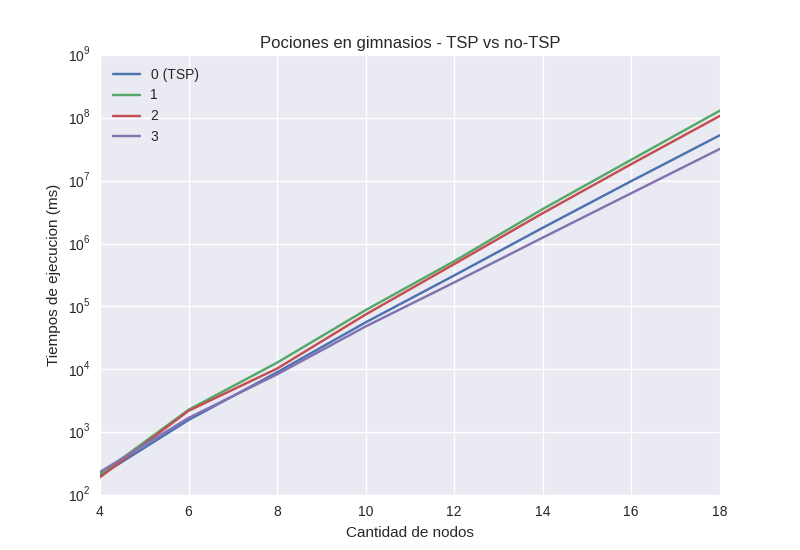
\includegraphics[width=\textwidth]{img/ejercicio1/exp5_1.png}
		\caption{Resultados del experimento 4.}
		\label{fig: ej1_exp5_1}
	\end{center}
\end{figure}

\par En la figura \ref{fig: ej1_exp5_1} podemos ver los resultados del experimento 4. Podemos notar que el caso TSP y el caso con 3 $Pociones necesarias$ se diferencian de los otros dos casos, tomando menor tiempo de ejecución. Notamos que el caso 3 es muy favorable, a diferencia de los 1 y 2. Creemos que esto se debe a que al necesitarse más pociones para ir a los gimnasios se realizan más podas que limitan la cantidad de instancias visitadas. Para esto, vamos a indagar más en el tema y compararemos los siguientes datos:

\begin{itemize}
	\item Cantidad de instancias visitadas: es la cantidad de instancias que se visitaron, sin importar si se calculó este valor o no.
	\item Cantidad de instancias calculadas: es la cantidad de instancias para las cuales se calculó la distancia mínima.
	\item Cantidad de podas del tipo 1: las podas del tipo 1 son: parar si no quedan más gimnasios; no ir a parada si tiene la mochila llena.
	\item Cantidad de podas del tipo 2: las podas del tipo 2 son: si la distancia al siguiente nodo es mayor que la distancia mínima parcial de la instancia no va a ese nodo; si la distancia al siguiente nodo es mayor que la distnacia mínima parcial global no va a ese nodo.
\end{itemize}

\newcolumntype{C}[1]{>{\centering\let\newline\\\arraybackslash\hspace{0pt}}m{#1}}

\begin{table}[h]
	\centering
	\rowcolors{2}{blue!10}{white}
	\begin{tabular}{|C{2cm}|C{2cm}|C{2cm}|C{2cm}|C{2cm}|C{2cm}|}
		\hline
		\rowcolor{gray!30}
		Cantidad de nodos & Pociones Gimnasio &  Cantidad de instancias visitadas &  Cantidad de instancias calculadas &  Cantidad de podas 1 &  Cantidad de podas 2 \\
		\hline
		4 &           0 (TSP) &                              13.0 &                               11.0 &                  2.5 &                  1.5 \\
		\hline
		4 &                 3 &                              20.5 &                               15.5 &                  4.0 &                  1.0 \\
		\hline
		6 &           0 (TSP) &                             160.0 &                               80.5 &                  5.0 &                  5.5 \\
		\hline
		6 &                 3 &                             182.5 &                               90.0 &                 18.0 &                  3.5 \\
		\hline
		8 &           0 (TSP) &                            1345.0 &                              449.0 &                  7.0 &                  7.0 \\
		\hline
		8 &                 3 &                            1258.5 &                              448.0 &                 88.0 &                  1.5 \\
		\hline
		10 &           0 (TSP) &                            9220.0 &                             2305.0 &                  9.0 &                  6.0 \\
		\hline
		10 &                 3 &                            7494.5 &                             2100.0 &                425.0 &                  0.5 \\
		\hline
		12 &           0 (TSP) &                           56309.0 &                            11264.5 &                 11.0 &                 22.5 \\
		\hline
		12 &                 3 &                           41113.0 &                             9504.0 &               1986.0 &                  5.0 \\
		\hline
		14 &           0 (TSP) &                          319431.0 &                            53247.5 &                 13.0 &                 69.5 \\
		\hline
		14 &                 3 &                          213665.5 &                            42042.0 &               9016.0 &                 16.5 \\
		\hline
		16 &           0 (TSP) &                         1720300.0 &                           245760.5 &                 15.0 &                 35.5 \\
		\hline
		16 &                 3 &                         1068495.5 &                           183040.0 &              40048.0 &                  8.5 \\
		\hline
		18 &           0 (TSP) &                         8912894.0 &                          1114113.0 &                 17.0 &                 20.0 \\
		\hline
		18 &				 3 &                         5191762.0 &                           787644.0 &             175041.0 &                  5.0 \\
		\hline
	\end{tabular}
	\caption{Datos de las corridas de casos TSP vs casos 3 pociones.}
	\label{tab: ej1_exp5_2}
\end{table}

\par En el cuadro \ref{tab: ej1_exp5_2} podemos ver los datos de las corridas de cada caso de entrada. Notamos que, para cualquier cantidad de nodos de entrada, la cantidad de instancias visitadas y la cantidad de instancias calculadas difieren mucho entre TSP y no-TSP. Este se condice diréctamente con la diferencia que se ve en la cantidad de podas del tipo 1. Esto se lo adjudicamos al hecho de que, para el caso de TSP, todos los nodos son de tipo gimnasio (excepto el primero). Por esto, no se realiza ninguna poda, todo camino es válido. Mientras que en el caso de no-TSP, se realizan muchas podas por no tener pociones suficientes para ir a algún gimnasio.

\par Finalmente, podemos comprender el por qué de las diferencias a favor del caso con $pociones necesarias = 3$. Vemos entonces que el caso TSP es simplemente un caso más, y no se trata de un mejor ni peor caso.

\medskip

\par De esta manera podemos concluir que estamos conformes con la forma en que pudimos disminuír los tiempos de ejecución del algoritmo, pero creemos que se podría haber probado una versión sin instancias, y que tenga libertad de podar teniendo en cuenta el camino previo (algo que la instancia planteada no nos permite).

\newpage

\section{Ejercicio 2: Heurística constructiva golosa}
\subsection{Introducción y descripción del algoritmo}
\par En este ejercicio se nos pide implementar una heurística constructiva golosa para resolver el juego.

\par El algoritmo goloso se basa en priorizar ciertos valores del grafo para recorrerlo. En este caso usamos la distancia entre los nodos y buscamos siempre el nodo válido más cercano para saltar a el.
	 	
\par La idea intuitiva es que minimizando la distancia entre cada salto de nodo a nodo se puede llegar a encontrar la mejor solución, cosa que en general no vale. 
	La ventaja es que es fácil de implementar y tiene complejidad polinomial.

\subsection{Idea general del algoritmo}

\par Hay dos tipos de nodos: gimnasios y paradas. Un jugador puede ir de un nodo a cualquier otro que no haya visitado antes. Por lo que solo nos manejaremos con una lista de todos los nodos del grafo . Entre dos nodos cualesquiera existe una distancia, que calcuaremos al inicio. También es importante notar que para ir a un nodo de tipo gimnasio se debe contar con al menos la cantidad de pociones necesarias para vencerlo. Pero al comenzar el jugador no cuenta con ninguna, por lo que el primer nodo ha visitar siempre debe ser uno del tipo parada.

\par Aclarados estos detalles, retomaremos el ejemplo mostrado en la descripción general del problema (figura \ref{fig: descripcion_ejemplo_entrada}), veremos las distancias entre estos nodos y analizaremos el funcionamiento del algoritmo sobre este caso en particular.

\begin{table}[h]
	\centering
	\begin{tabular}{|>{\centering\arraybackslash}p{2cm}|>{\centering\arraybackslash}p{2cm}|>{\centering\arraybackslash}p{2cm}|>{\centering\arraybackslash}p{2cm}|>{\centering\arraybackslash}p{2cm}|}
		\hline
		   & \textbf{G1} & \textbf{G2} & \textbf{P1} & \textbf{P2} \\ \hline
		\textbf{G1} & \cellcolor{gray} & 1.41421 & 2.82842 & 2 \\ \hline
		\textbf{G2} & 1.41421 & \cellcolor{gray} & 1.41421 & 1.41421 \\ \hline
		\textbf{P1} & 2.82842 & 1.41421 & \cellcolor{gray} & 2 \\ \hline
		\textbf{P2} & 2 & 1.41421 & 2 & \cellcolor{gray} \\
		\hline
	\end{tabular}
	\caption{Distancias entre los nodos del caso de ejemplo.}
	\label{fig: ejercicio1_ejemplo_distancias}
\end{table}

\par El algoritmo se basa en recorrer nodo por nodo siempre yendo al vecino más cercano, priorizando los nodos gimnasio si tiene las pociones necesarias para ir a el. Es decir, si puede ir a un nodo gimnasio y a un nodo parada, va a ir al nodo gimnasio. En otro caso va a una parada a buscar más pociones.
\par Al tomar este ejemplo de entrada, el algoritmo comenzará parándose sobre algún nodo \textit{i} del tipo parada (en particular, nos paramos en la pokeparada más cercana al primer gimnasio de la entrada) y calculará el camino goloso partiendo desde él. En el ejemplo, comienza por el nodo \textit{P2}, ya que es la parada más cercana al primer gimnasio \textit{G1}.

\begin{figure}[H]
    \begin{subfigure}[b]{0.49\textwidth}
        \includegraphics[width=\linewidth]{img/ejercicio2/ejercicio1_ejemplo_camino1_2.png}
        \caption{Camino exacto.}
        \label{fig: ejercicio1_ejemplo_camino1_2}
    \end{subfigure}
    \begin{subfigure}[b]{0.49\textwidth}
        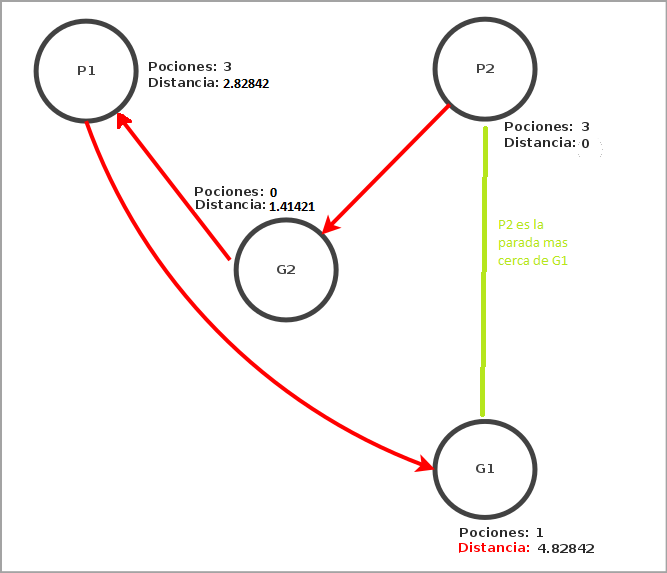
\includegraphics[width=\linewidth]{img/ejercicio2/ejercicio1_ejemplo_camino1_4.png}
        \caption{Camino con algoritmo goloso.}
        \label{fig: ejercicio1_ejemplo_camino1_4}
    \end{subfigure}
    \caption{Camino exacto calculado con backtracking y camino goloso}
    \label{fig: ejercicio1_ejemplo_caminos1}
\end{figure}


\subsection{Explicación del algoritmo}

\par Para nuestro algoritmo goloso tenemos la matriz de distancias del grafo con los nodos que nos pasaron en la entrada


\par La función que calcula el camino goloso recibe los siguientes parámetros:
\begin{itemize}
\item distancias: Es una matriz de distancias ya calculadas a partir de la entrada.
\item gimnasios\_costo : Es un vector que en cada índice $i$ tiene la cantidad de pociones que cuesta matar al gimnasio $i$
\item gimnasios\_totales : Tiene la cantidad total de gimnasios pasador por parámetro.
\end{itemize}
\par El algoritmo es iterativo y tiene la siguiente estructura:

\begin{itemize}
	\item Primero calcula la pokeparada más cercana al primer gimnasio de la entrada y la guarda como el primer nodo a recorrer así como el primer nodo de la solución.
	\item Luego entra en un ciclo que dura mientras la cantidad de gimnasios que recorrimos sea menor a la cantidad total de gimnasios.
	\item Dentro de este ciclo principal se entra en otro ciclo que itera sobre todos los gimnasios para tomar el gimnasio más cercano al nodo actual. Se va tomar el gimnasio más cercano tal que no se haya recorrido y se tengan las pociones necesarias para poder matarlo.
	\item Al salir del ciclo secundario anterior, el algoritmo se fija si encontró algún nodo gimnasio para tomar como el siguiente. En el caso de que no lo haya encontrado hay que iterar de forma similar para encontrar la pokeparada más cercana y sumar las pociones, si no encuentra pokeparada entonces no hay solución al problema y se sale del ciclo principal.
	\par Si encontró un gimnasio se restan las pociones gastadas para matarlo y se suma $uno$ en el contador de gimnasios recorridos. 
\par Por último agrega el nodo que haya encontrado al camino solución.
	\item Una vez afuera del ciclo principal el algoritmo chequea si se recorrieron todos los gimnasios. En caso afirmativo simplemente itera sobre el camino para calcular la distancia recorrida y devolverla. En el otro caso se devuelve un $-1$, ya que no se pudieron matar todos los gimnasios.
\end{itemize}

\medskip

\SetAlgoLined
\SetKwProg{Fn}{Function}{:}{EndFunction}
\begin{algorithm}[H]
	\label{algo: ejercicio2_pseudocodigo}
	\Fn{camino\_goloso(distancias : Matriz(int)), gimnasios\_costo : vector(int), gimnasios\_totales : int}{
		$solucion\_res :$ vector(int)	
		\BlankLine
		$gimnasios\_recorridos \gets$ 0	
		\BlankLine	
		$pocionesActuales \gets$ 0
		\BlankLine
		$distancia\_res \gets 0$
		\BlankLine
		$nodo\_actual \gets $ PokeParadamásCercana(primer gimnasio) \Comment{$O(m) $}
		\BlankLine
		solucion\_res.push(nodo\_actual);
		\BlankLine
		\While{gimnasios\_recorridos $<$ gimnasios\_totales} { 
			\BlankLine
			$gimnasio\_cercano \gets$ -1
			\BlankLine
			\For{gym\_i $<$ gimnasios\_totales; gym\_i++} {
		\BlankLine
		$minimo \gets$ $\infty$
\BlankLine
		\If{ minimo $>$ distancias[gym\_i][nodo\_actual]
           	$\&$    pocionesActuales $\geq$ gimnasios\_costo[gym\_i]) 
             $\&$  NoLoRecorri(gym\_i)}
              {		\BlankLine
			$minimo \gets$ distancias[gym\_i][nodo\_actual]		\BlankLine
                $gimnasiocercano \gets$ gym\_i 		\BlankLine
              }		\BlankLine

			}		\BlankLine		\BlankLine
		
	\If{No encontr\'e gimnasio para matar}{		\BlankLine

       \If{No hay más pokeparadas}{ 		\BlankLine
          break;
        } 			
	       \Else {$nodoActual \gets$ pokeparadamásCercana(nodo\_actual)
			\BlankLine
          $pocionesActuales \gets$ pocionesActuales + 3
	
        }		\BlankLine
      }		\BlankLine
	\Else{ %mato el gimnasio!		
		\BlankLine
        $gimnasios\_recorridos \gets gimnasios\_recorridos + 1$		\BlankLine
        $nodoActual \gets$ gimnasiocercano		\BlankLine
       $ pocionesActuales \gets pocionesActuales - gimnasios\_costo[nodoActual]$		\BlankLine
      }		\BlankLine
      $solucion\_res.push(nodoActual+1)$		\BlankLine
    }	\BlankLine

    \If{gimnasios\_recorridos $<$ gimnasios\_totales} {		\BlankLine		\BlankLine
     %-distancia invalida
      distancia\_res = -1;
    } \Else {		\BlankLine
      $distancia\_res \gets$ CalcularDistancia(solucion\_res)
      }		\BlankLine
		\BlankLine
	return solucion\_res, distancia\_res
}
	

\end{algorithm}



\subsection{Análisis de complejidad}

\par Para analizar la complejidad del algoritmo y su implementación debemos definir ciertos conceptos y parámetros:

\begin{itemize}
	\item \textbf{n}: Cantidad de nodos del tipo gimnasio.
	\item \textbf{m}: Cantidad de nodos del tipo parada.
	\item \textbf{k}: Capacidad de la mochila del jugador.
\end{itemize}



\begin{itemize}
	\item Buscar la pokeparada más cercana al primer gimnasio consiste en un loop que itera sobre las pokeparadas y se queda con la más cercana, eso cuesta O($m$)
	\item El loop principal puede llegar a iterar todos los nodos del grafo, O($n + m$)
	\item Luego viene el loop anidado sobre el anterior e itera sobre los gimnasios, cuesta O($n$). 
	\item En caso de no haber encontrado gimnasio busca pokeparada más cercana, O($m$). Esto es dentro del loop principal , pero fuera del anterior.
	\item Sobre el final, ya fuera de los loops, se itera sobre el camino que quedó para sacar la distancia total, cuesta O($m + n$)
\end{itemize}

\par Vemos que en total todo cuesta O($m$ $+$ $(m+n)^2$ $+$ $m + n$) = O(\textit{max}($m^2, n^2, m*n$)). Vemos más en detalle esta cota:

\begin{equation}
	max(m^2, n^2, m*n)
\end{equation}
tenemos
\begin{equation}
	si\ |m| > |n| \Rightarrow max(m^2, n^2, m*n) = m^2
\end{equation}
\begin{equation}
	si\ |m| < |n| \Rightarrow max(m^2, n^2, m*n) = n^2
\end{equation}
\begin{equation}
	si\ |m| = |n| \Rightarrow max(m^2, n^2, m*n) = m^2 = n^2
\end{equation}
Entonces podemos decir que 
\begin{equation}
	max(m^2, n^2, m*n) = max(m^2, n^2)
\end{equation}

\par De esta manera podemos concluir que la complejidad total del algoritmo es \textbf{O($max(m^2, n^2)$)}.

\subsection{La solución no siempre es la mejor}
	En las imágenes siguientes, la doble flecha negra indica la distancia entre los nodos, y la flecha roja el camino elejido:
\begin{figure}[H]
    \begin{subfigure}[b]{0.49\textwidth}
        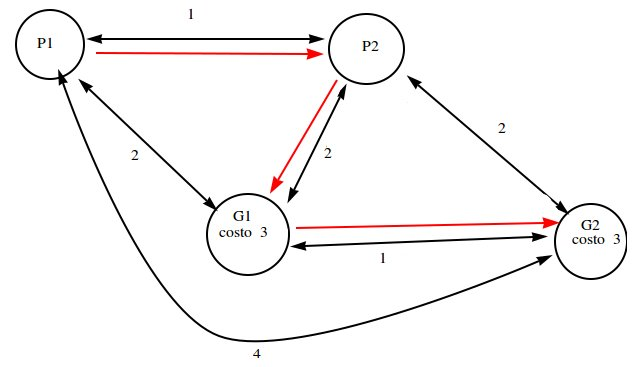
\includegraphics[width=\linewidth]{img/ejercicio2/exacto.jpg}
        \caption{Camino exacto.}
        \label{fig: ejercicio1_ejemplo_camino1_2}
    \end{subfigure}
    \begin{subfigure}[b]{0.49\textwidth}
        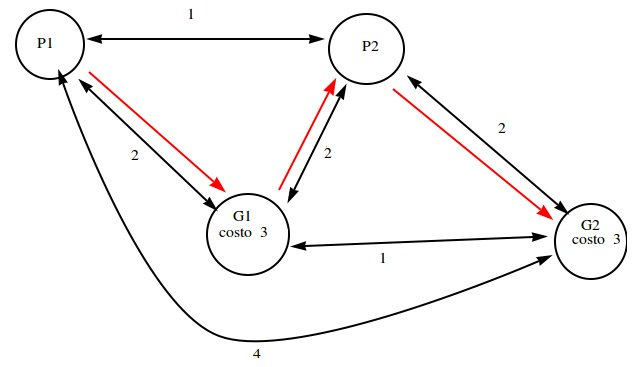
\includegraphics[width=\linewidth]{img/ejercicio2/goloso_malo.jpg}
        \caption{Camino con algoritmo goloso.}
        \label{fig: ejercicio1_ejemplo_camino1_4}
    \end{subfigure}
    \caption{Camino exacto calculado con backtracking y camino goloso}
    \label{fig: ejercicio1_ejemplo_caminos1}
\end{figure}

Como se ve, en el camino exacto la distancia total es $4$, mientras que en el goloso es $6$. 
Esto es en parte a que el goloso empieza en una pokeparada definida y además solo optimiza la distancia localmente, tal vez perdiendo una mejor arista para tomar en otro nodo no vecino al actual.

\subsection{Experimentación}
%	La complejidad del algoritmo es O(\textit{max}($m^2, n^2, m*n$)). Por lo tanto mostramos dos graficos, uno variando la cantidad de gimnasios y otro variando la cantidad de pokeparadas, de 0 a 10:
%	\begin{figure}[H]
%    \begin{subfigure}[b]{0.49\textwidth}
%        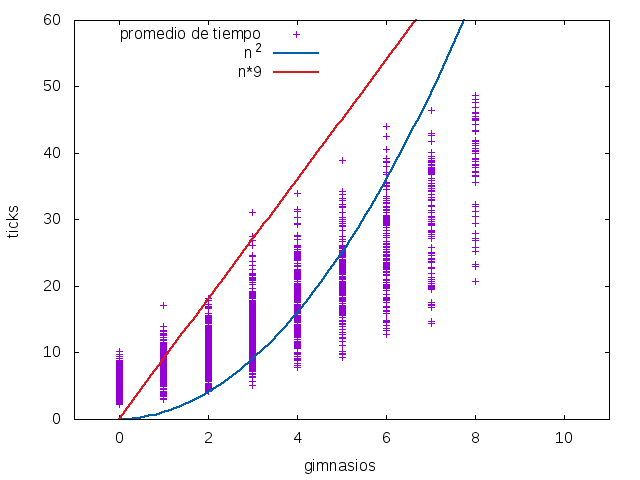
\includegraphics[width=\linewidth]{img/ejercicio2/salidaN.png}
%        \caption{Grafico variando los gimnasios.}
%        \label{fig: ejercicio1_ejemplo_camino1_2}
%    \end{subfigure}
%    \begin{subfigure}[b]{0.49\textwidth}
%        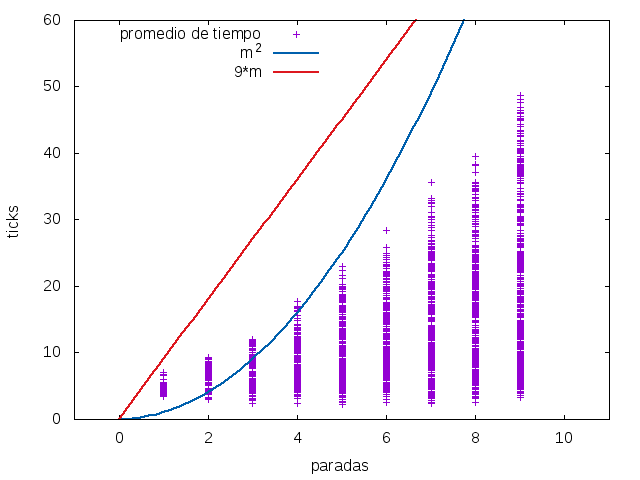
\includegraphics[width=\linewidth]{img/ejercicio2/salidaM.png}
%        \caption{Grafico variando las pokeparadas.}
%        \label{fig: ejercicio1_ejemplo_camino1_4}
%    \end{subfigure}
%    \label{fig: ejercicio1_ejemplo_caminos1}
%\end{figure}
%
%Por cada $x$ del dominio tenemos 10 cruces, que son los tiempo de ejecución habiendo fijado ese x y moviendo la otra variable. Es decir, si en el gráfico de gimnasios tomamos $gimnasios = 2$, tenemos los tiempo de ejecución de $( gimnasios = 2, paradas = 0...9) $. 
%
%\par Como la complejidad viene en función de un máximo, graficamos cada candidato a máximo y vemos que cada uno es más grande que los tiempos de ejecución.
%\par En el caso de O$(n*m)$ graficamos la funciòn $9 * m$ o $n * 9$, que es el máximo valor que puede llegar a tomar en nuestro muestreo.
%
%\par En ambos casos se ve como la complejidad tiene una tendencia mayor a los tiempos de ejecución.
%\\
%En el siguiente gráfico variamos la mochila fijando las otras variables:
%	\begin{figure}[H]
%    \begin{subfigure}[b]{0.49\textwidth}
%        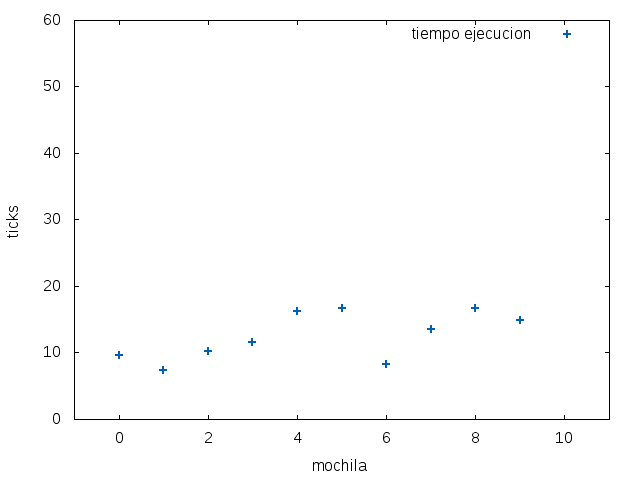
\includegraphics[width=\linewidth]{img/ejercicio2/salidaMochifijadaM.png}
%        \caption{Grafico variando las mochilas.}
%        \label{fig: ejercicio1_ejemplo_camino1_2}
%    \end{subfigure}
%    
%    \label{fig: ejercicio1_ejemplo_caminos1}
%\end{figure}
%
%En este caso la función no tiene una tendencia a crecer. Esto es lo que se esperaba, ya que la complejidad no depende de la amplitud de la mochila, por lo tanto los tiempos de ejecución deberían mantenerse en orden constante al variar la mochila.


%\begin{figure}[H]
%  \begin{center}
%    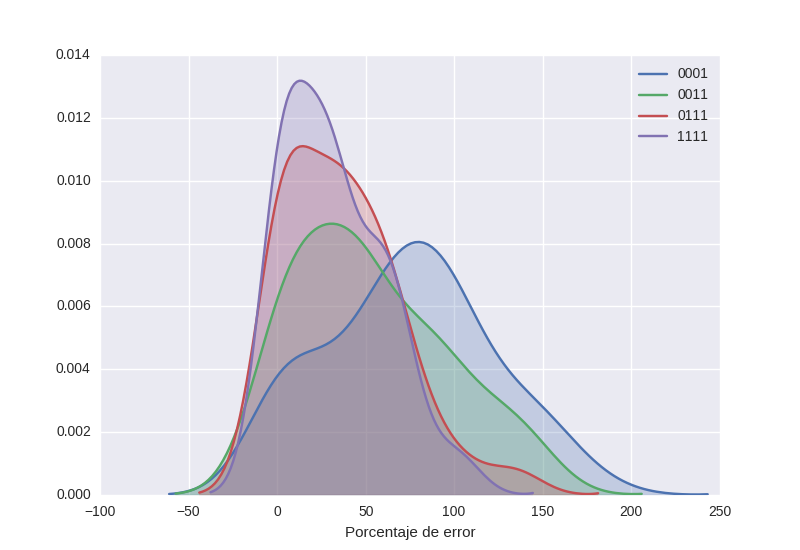
\includegraphics[width=\textwidth]{img/ejercicio3/exp3_distribuciones.png}
%    \caption{Distribución de los porcentajes de error sobre casos con solución válida.}
%    \label{fig: ej3_exp3_an1_distr_validados}
%  \end{center}
%\end{figure}

En esta sección vamos a ir mostrando y explicando los resultados de cada experimento que propusimos.
En resumen vamos a ir variando cada una de las variables e ir comparando tiempos con respecto a cada una de ellas, es decir, vamos a ir variando; capacidad de mochila, cantidad de paradas y cantidad de gimnasios.

\subsubsection{Experimento 1: Cantidad de Gimnasios vs Tiempos de ejecución}

En el siguiente gráfico fijamos la mochila y variamos la cantidad de gimnasios, sin usar escala logarítmica:

\begin{itemize}
\item Cantidad de paradas = 100.
\item Capacidad mochila = 20.
\item La cantidad de pociones necesarias en cada gimnasio es random.
\end{itemize}


\begin{figure}[H]
  \begin{center}
    \begin{subfigure}[b]{0.70\textwidth}	
        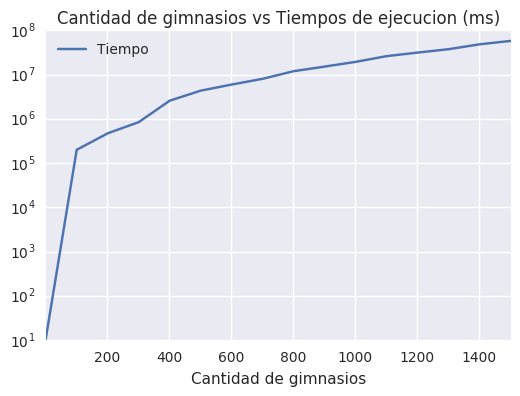
\includegraphics[width=\textwidth]{img/ejercicio2/losPosta/grafico_gimnasios.png}
        \caption{Gráfico variando cantidad de gimnasios.}
        \label{fig: ejercicio1_ejemplo_camino1_2}
    \end{subfigure}
  \end{center}
\end{figure}


Podemos ver como se comportan los tiempos a medida que vamos aumentando la cantidad de gimnasios, en si los valores no son tan importantes.
Ya que a la larga deberia ser el mismo crecimiento, por como se comporta nuestro algoritmo, es decir, sabemos que siempre va a ir a buscar una parada más cerca y
en caso de poseer suficientes posiciones para atacar un gimnasio, lo hace. Por más que tengamos una amplia mochila o tengamos muchas pokeparadas, lo que importa es la cantidad de gimnasios y
la cantidad de pociones que necesitamos para atacarlo. Si tenemos gimnasios con el requisito de posiciones en valores altos, el tiempo va a ser mayor ya que va a requerir de recorrer más nodos para poder derrotarlos.
Lo interesante del gráfico es su semejanza a una funcion logaritimica. No sabemos exactamente porque de este comportaminto, pero nos dios la 
sensacion de que en funcion de los gimnasios solamente el algoritmo, a la larga, tiene tiempos logartimos en funcion de los gimnasios.


\subsubsection{Experimento 2: Cantidad de paradas vs Tiempos de ejecución}

\begin{itemize}
\item Cantidad Gimnasios = 50.
\item Capacidad de la mochila = 200.
\item La cantidad de pociones necesarias en cada gimnasio es random.
\end{itemize}

Esta vez vamos a mostrar como se comporta nuestro algoritmo en terminos de tiempo al aumentar la cantidad de paradas y dejar fija la capacidad de la mochila y la cantidad de gimnasios:

\begin{figure}[H]
  \begin{center}
    \begin{subfigure}[b]{0.70\textwidth}
        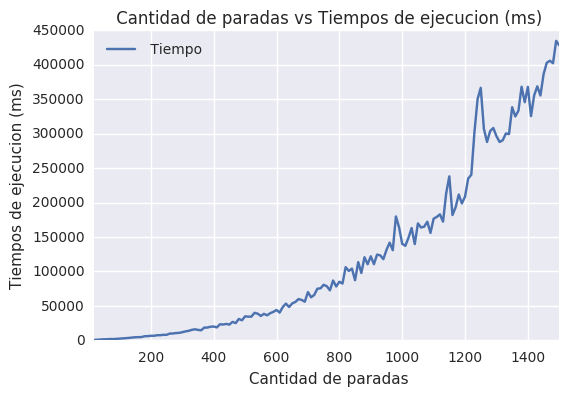
\includegraphics[width=\textwidth]{img/ejercicio2/losPosta/grafico_sin_logs.png}
        \caption{Gráfico variando la cantidad de paradas.}
        \label{fig: ejercicio1_ejemplo_camino1_2}
   \end{subfigure}
  \end{center}
\end{figure}


El mismo gráfico con escala logartimica en el eje y:
\begin{figure}[H]
  \begin{center}
    \begin{subfigure}[b]{0.70\textwidth}
        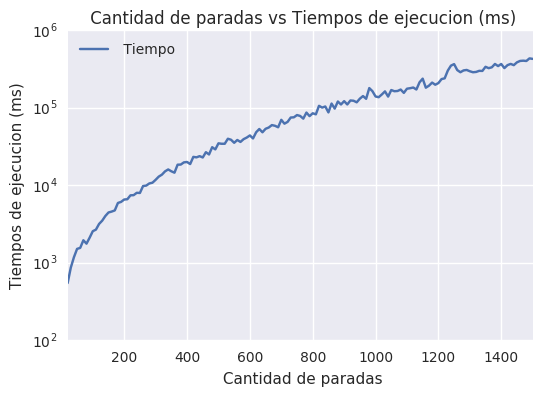
\includegraphics[width=\textwidth]{img/ejercicio2/losPosta/grafico_log_y.png}
        \caption{Grafico variando la cantidad de paradas escala logarimica en eje y.}
        \label{fig: ejercicio1_ejemplo_camino1_2}
   \end{subfigure}
  \end{center}
\end{figure}

Y por último el mismo grafico pero aplicando la escala en ambos ejes:

\begin{figure}[H]
  \begin{center}
   \begin{subfigure}[b]{0.70\textwidth}	
        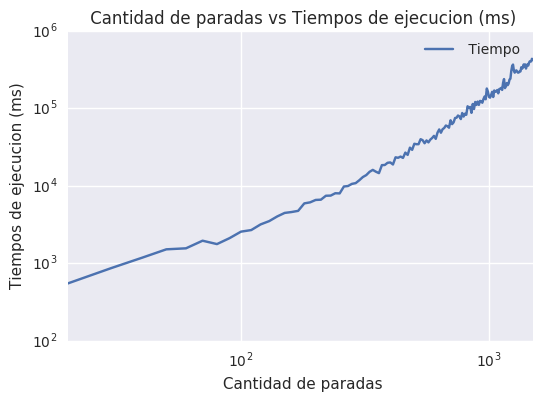
\includegraphics[width=\textwidth]{img/ejercicio2/losPosta/grafico_con_2_logs.png}
        \caption{Grafico variando la cantidad de paradas escala logarimica en x e y.}
        \label{fig: ejercicio1_ejemplo_camino1_2}
   \end{subfigure}
  \end{center}
\end{figure}

En estos gráficos podemos ver como se comporta nuestro algoritmo cuando fijamos la cantidad de gimnasios y la capacidad de la mochila, y variamos la cantidad de paradas en funcion del tiempo.
Podemos observar que a medida qeu las paradas son mayores, las corridas son más largas haciendo que el tiempo aumente de forma exponencial.
Esto igualmente tiene muchas varibles, pero en nuestro caso al aumentar la cantidad de pokeparadas, estamos aumentando los tiempso de ejecucion ya que, cada vez que querramos visitar el proximo nodo
vamos a necesitar saber las distancias de todos los nodos con respecto al que estamos parados, haciendo que la complejidad temporal suba considerablemente.

\subsubsection{Experimento 3: Capacidad de la mochila vs Tiempos de ejecución}

Nos queda por mostrar como varian los tiempos al variar la capacidad de la mochila y dejar fijos ambos valores de paradas y gimnasios:

\begin{itemize}
\item Cantidad de Gimnasios = 50.
\item Cantidad de pokeparadas = 100.
\end{itemize}

\begin{figure}[H]
  \begin{center}	
    \begin{subfigure}[b]{0.70\textwidth}
        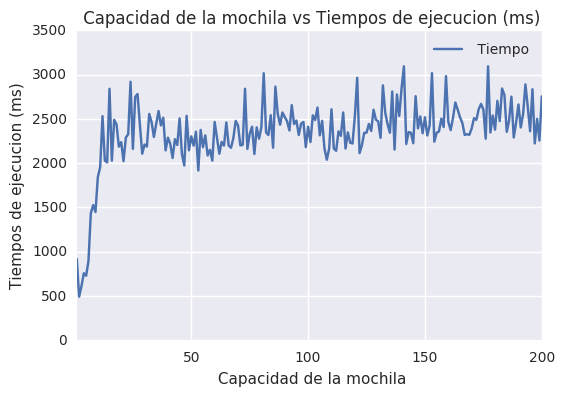
\includegraphics[width=\textwidth]{img/ejercicio2/losPosta/grafico.png}
        \caption{Gráfico variando la capacidad de la mochila.}
        \label{fig: ejercicio1_ejemplo_camino1_2}
 \end{subfigure}
  \end{center}
\end{figure}

En este gráfico vemos como se comporta el goloso al variar la capacidad de la mochila y dejar fija la cantidad de pokeparadas y gimnasios.
Como se observa el comportambien es parecido por más que aumentemos la capacidad de la mochila, creemos que esto tiene bastante sentido ya que
aumentar la capacidad solo hace que pueda llevar más posiones, pero por como actua nuestro goloso, si en algun momento tiene las suficientes posiones como para ir a 
derrotar un gimnasio, lo va a ir a hacer. Entonces lo que permite esto es no aprovechar cantidades muy grandes de capacidad de mochila, ya que igualmente (si a priori puede) va a ir al gimnasio con menor
requisito de pociones. Luego el gráfico no debería variar demasiado entre instancias distintas de este tipo.

\subsubsection{Experimento 4: Cantidad de Gimnasios vs Tiempos de ejecución TSP}

Ahora mostramos el caso tsp fijando mochila y paradas, pero variando la cantidad de gimnasios.

\begin{itemize}
\item Cantidad de paradas = 100.
\item Capacidad de la mochila = 20.
\item La cantidad de pociones necesarias en cada gimnasio es random.
\end{itemize}

\begin{figure}[H]
  \begin{center}	
    \begin{subfigure}[b]{0.49\textwidth}
        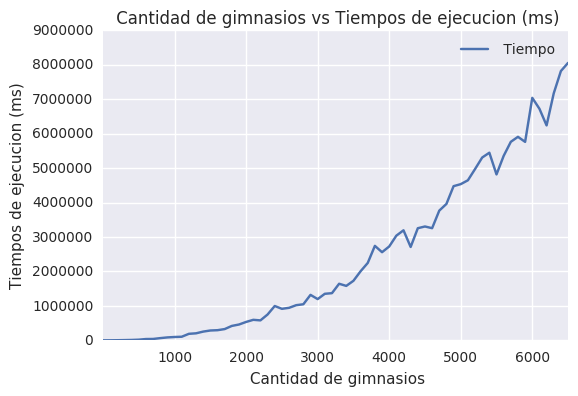
\includegraphics[width=\textwidth]{img/ejercicio2/losPosta/grafico_sin_log.png}
        \caption{Gráfico variando las mochilas.}
        \label{fig: ejercicio1_ejemplo_camino1_2}
 \end{subfigure}
 
    \begin{subfigure}[b]{0.49\textwidth}
        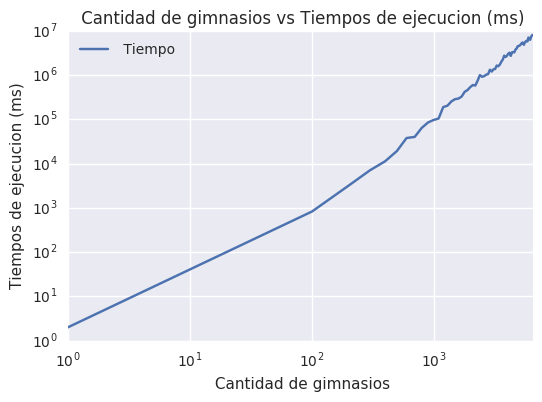
\includegraphics[width=\textwidth]{img/ejercicio2/losPosta/grafico_2log.png}
        \caption{Gráfico variando la cantidad de gimnasios con escala logarimica en x e y.}
        \label{fig: ejercicio1_ejemplo_camino1_2}
  \end{subfigure}

  \end{center}
\end{figure}
 	  
\begin{figure}[H] 
 \begin{center}
	\begin{subfigure}[b]{0.59\textwidth}
        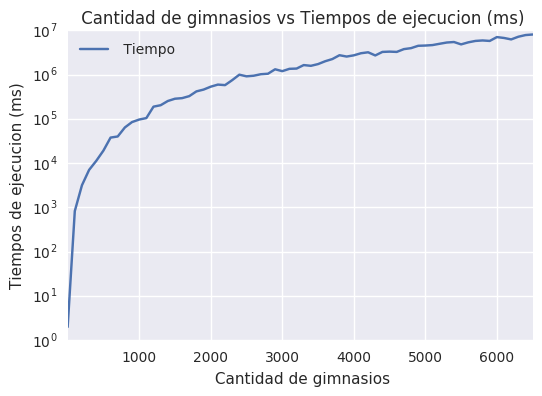
\includegraphics[width=\textwidth]{img/ejercicio2/losPosta/grafico_logy.png}
        \caption{Gráfico variando la cantidad de mochilas con escala logaritmica en eje y.}
        \label{fig: ejercicio1_ejemplo_camino1_2}
 \end{subfigure}
  \end{center}
\end{figure}

Este gráfico muestra el rendimiento del goloso con tsp, podemos observa con relación al primer gráfico que mostramos en esta sección.
que su crecimento a medida que vamos aumentando los gimnasios es de tipo exponencial.

\subsubsection{Experimento 5: Comparacion entre los tiempos vs complejidad ($n^2$) y ($n^3$) }

\begin{figure}[H]
  \begin{center}	
    \begin{subfigure}[b]{0.60\textwidth}
        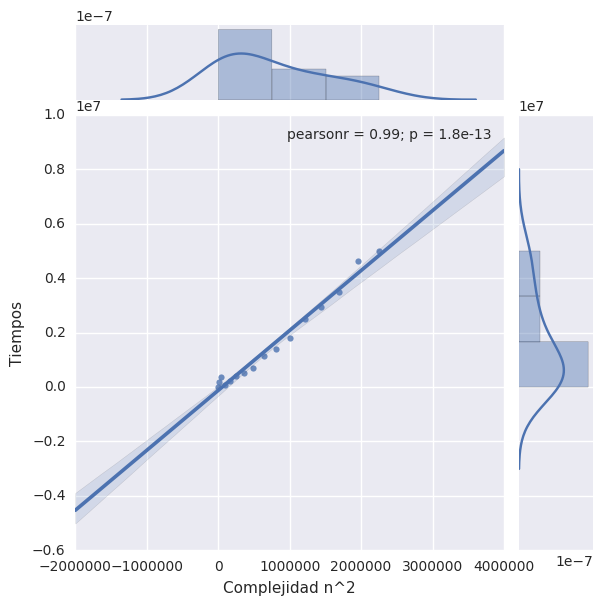
\includegraphics[width=\textwidth]{img/ejercicio2/losPosta/pearsonncuadrado.png}
        \caption{Gráfico variando las mochilas.}
        \label{fig: ejercicio1_ejemplo_camino1_2}
 \end{subfigure}
 
    \begin{subfigure}[b]{0.60\textwidth}
        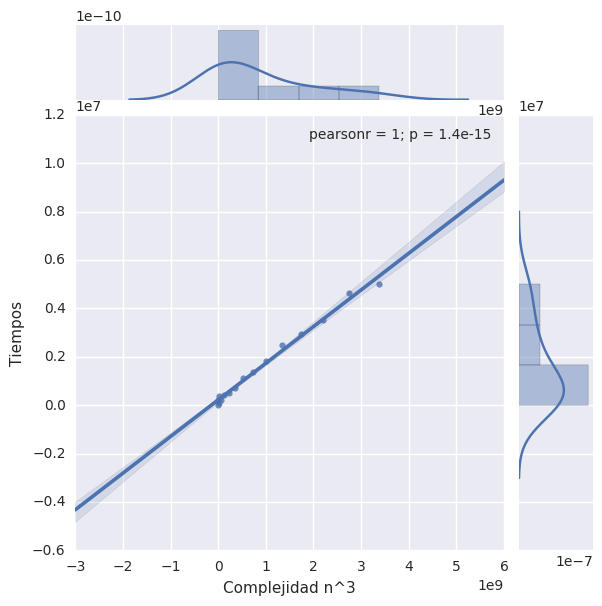
\includegraphics[width=\textwidth]{img/ejercicio2/losPosta/pearsonncubo.png}
        \caption{Gráfico variando la cantidad de gimnasios con escala logarimica en x e y.}
        \label{fig: ejercicio1_ejemplo_camino1_2}
	   \end{subfigure}

  \end{center}
\end{figure}

En el gr\'afico se puede ver una muy buena correlaci\'on entre los tiempos obtenidos en las corridas y una funci\'on cuadr\'atica. Esta observaci\'on la pudimos realizar debido a que el coeficiente de Pearson es 0.99 y su $valor p$ es muy pequeño. De esta manera podemos afirmar que nuestra cota de complejidad estaba bien calculada.


\subsubsection{Experimento 6: Evaluacion de calidad de la solucion con porcentaje de error }

\begin{figure}[H]
  \begin{center}	
    \begin{subfigure}[b]{0.60\textwidth}
        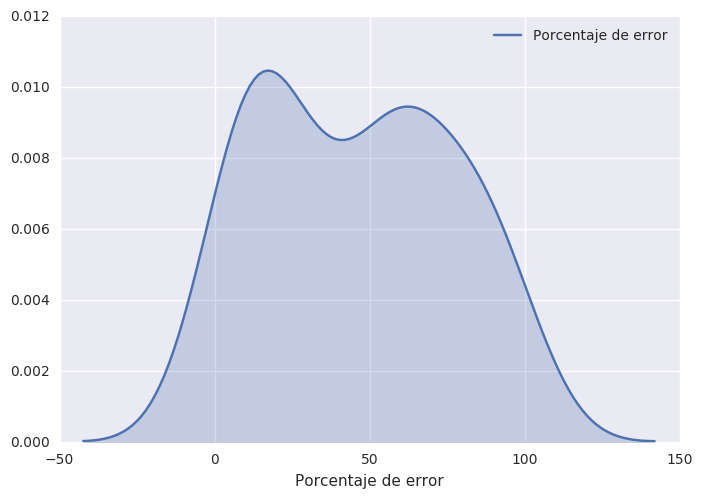
\includegraphics[width=\textwidth]{img/ejercicio2/losPosta/grafico_distribucion.png}
        \caption{Comparacion de calida de la solucion.}
        \label{fig: ejercicio1_ejemplo_camino1_2}
    \end{subfigure}
  \end{center}
\end{figure}

En la figura podemos observar que el error del algoritmo suele variar m\'as que nada entre 25\% y el 75\% de la soluci\'on exacta. Este resultado nos va a servir como cota superior del error de los resultados de la heur\'istica y la metaheur\'istica.

\newpage
\section{Ejercicio 3: Heurística de búsqueda local}
\subsection{Introducción}

En este punto vamos a aplicar la heurística de búsqueda local para intentar mejorar la solución a partir de una solución particular, vamos a mostrar cómo armamos los conjuntos de vecindades y cómo aplicamos el algoritmo para descubrir una solución mejor a la solución que teníamos inicialmente.

La idea básica de los algoritmos de búsqueda local es la siguiente, en general la idea siempre es la misma:

\begin{itemize}
  \item Iniciar con una solución generada aleatoriamente o hallada con algún otro algoritmo.
  \item Aplicar a la solución actual una transformación de algún conjunto dado de transformaciones para mejorar la solución (vecindades).
  \item La solución mejorada se convierte en la solución actual, repetir hasta que ninguna transformación del conjunto mejore a la solución actual.
\end{itemize}

En nuestro caso, vamos a utilizar esta idea, pero para ello es necesario que nos definamos estas trasformaciones y podamos asi compararla con la solución inicial de la cual partimos.

En la figura \ref{fig: ej3_ejemplo_mejora} podemos ver un ejemplo de cómo el algoritmo de búsqueda local va mejorando la solución en función de las iteraciones del ciclo (épocas).

\begin{figure}[H]
  \begin{center}
    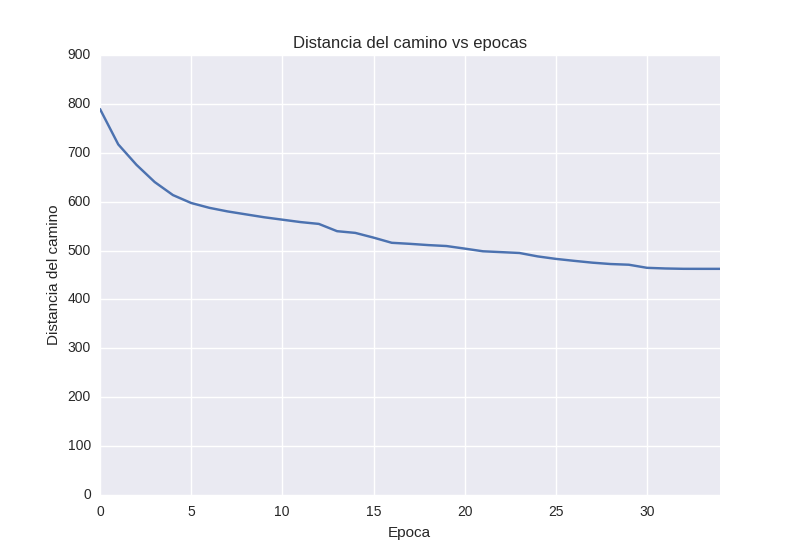
\includegraphics[width=\textwidth]{img/ejercicio3/ejemplo_cambios.png}
    \caption{Ejemplo del funcionamiento de la heurística de búsqueda local.}
    \label{fig: ej3_ejemplo_mejora}
  \end{center}
\end{figure}

\subsection{Explicación de la heurística de búsqueda local}
\label{sec: ej3_explicacion}

Para esta heurística presentamos 4 tipos de vecindades distintas, esto nos permite poder intentar mejorar una solución inicial. En nuestro caso comenzamos con un goloso, y vamos construyendo las distintas vecindades, luego elegimos alguna de ellas y buscamos la mejor solución que mejore la inicial.

\begin{itemize}

\item La primer vecindad va a estar compuesta por todas las soluciones que surjan de cambiar las pokeparadas que quedaron fuera de la solución con las que están dentro de la solución inicial, entonces por cada una de las paradas de la solución vamos a ir haciendo swap con una de las paradas que quedaron fuera, como estamos haciendo el cambio entre paradas no hace falta que revisemos si el camino resultante es válido.

\item La segunda está compuesta por las pokeparadas de la solución, es decir, vamos a ir intercambiando el orden de estas paradas dentro de la solución.

\item La tercera involucra a gimnasios y a pokeparadas, en esta vamos a ir intercambiando el orden de visita tanto de pokeparadas como de gimnasios, para ellos vamos a ir recorriendo la solución de principio a fin e intercambiando una pokeparada/gimnasio con el siguiente.

\item La última vecindad que planteamos se trata de intercambiar las posiciones de los gimnasios dentro de la solución, para ellos necesitamos que sea válido para tomarlo con un vecino posible.

\end{itemize}

En la primer vecindad, comenzamos por obtener una solución de una instancia por medio del algoritmo goloso. Partiendo de esta base, vamos a intentar intercambiar las paradas de esta solución con las pokeparadas que quedaron afuera y no son parte de la solución que devolvió el goloso. Para poder recorrer todas las pokeparadas dentro de la solución e ir intercambiandolas con las de afuera, tuvimos que quedarnos con las pokeparadas iniciales.
Esto nos permite poder saber rápidamente cuáles son las que no pertecen a la solución. Entonces, por cada una de las pokeparadas de la solución vamos a ir intercambiándola con alguna parada que quedó fuera, luego vamos a calcular la distancia total otra vez y compararla con la distancia total anterior (es decir, antes de que hagamos el intercambio de paradas) para quedarnos con alguna mejor.

Para la segunda vecindad, fuimos recorriendo cada pokeparada de la solución e intercambiándola con otra parada de la misma solución pero que se encuentre por delante, es decir como la solución viene ordenada para representar el camino, vamos a querer cambiar las paradas futuras y así establecer otro orden de visita de las mismas. Es por ello que cada vez que querramos intercambiar pokeparadas nos aseguramos que sean paradas de la solución y no gimnasios.

Para la tercera vecindad, lo único que tuvimos que hacer es recorrer la solución desde el principio al final e intercambiar los nodos. Cada nodo de la solución lo cambiamos con el siguiente y preguntamos si era una solución válida. Si era válida, entonces nos la guardamos.

La última vecindad lo que hacemos es intercambiar los gimnasios dentro de la misma solución entre ellos, para ello recorremos la solución y vamos intercambiando cada uno con los siguientes. Luego de cada cambio, verificamos si la solución es válida. En caso positivo, la guardamos. Luego, se vuelve el cambio atrás para continuar con otro cambio.


La búsqueda local en sí, se hace a partir de estas vecindades, en nuestro algoritmo tenemos una entrada que indica el tipo de vecindades que va a utilizar.
Esta entrada es de longitud 4 y se espera que este compuesta por algún '1' en el caso que se quiera hacer la búsqueda usando una vecindad. Pasamos a detallarlo mejor a continuación.
\begin{itemize}
\item entrada = '1xxx' Este tipo de entrada lo que indica es que se va hacer la búsqueda usando una sola vecindad, dicha vecindad es la primera que se indica más arriba.

\item entrada = 'x1xx' Este tipo de entrada indica que se hará la búsqueda sólo con la segunda vecindad.

\item entrada = 'xx1x' Se hará la búsqueda con la tercera vecindad.

\item entrada = 'xxx1' se hará la búsqueda con la cuarta vecindad.
\end{itemize}

Además de esto, también podemos combinar vecindades o utilizar todas. En el caso de utilizar todas, la entrada sería '1111'.
Lo que hacemos básicamente es observar qué vecindad o qué vecindades se indicaron para hacer la búsqueda, obtener todas esas soluciones vecinas y comparar cuál de ellas es la mejor y devolverla.

\subsection{Cota de complejidad}

Para el cálculo de complejidad vamos a usar siempre N, como cantidad de elementos totales de una instancia del problema, es decir, la suma de pokeparadas y gimnasios.

\subsubsection{Análisis de las vecindades}

\begin{itemize}

\item  Vecindad con las pokeparadas de los de afuera:

\begin{verbatim}
pokeNueva = 0;
pokeVieja = 0;
 Por cada N nodo en la solución
  Si N es una pokeparada 
   Por cada M nodo en las pokeparadas totales del la instancia
    Si M no esta en la solución
     Pokenueva = M;
     PokeVieja = N;
     Intercambio N por M en la solución nueva
     Me guardo en RESULTADO la solución que acabo de encontrar.
     Reestablezco la solución intercambiando M por N  
return RESULTADO;
\end{verbatim}

Al recorrer todos los nodos de la solución inicial tenemos un complejidad lineal en la cantidad de nodos de dicha solución$ O(N)$. Luego, por cada nodo de estos, necesitamos ver si es una pokeparada, lo cual se puede hacer de forma inmediata, ya que solo es ver que el valor del nodo sea menor a la cantidad de gimnasios totales, eso es $O(1)$. Luego iteramos por cada N (en el pseudocodigo) los M, que es un elemento del conjunto de las pokeparadas totales de la instancia. Por esta iteracion tenemos $O(N)$ en peor caso, donde N es la cantidad total de nodos de una instancia, pero luego como lo estamos haciendo para cada N, este doble ciclo tiene una complejidad de $O(N^2)$. Por ultimo, necesitamos también averiguar si la nueva solución que nos creamos al intercambiar dos paradas es válida, para ello tenemos que recorrer linealmente cada nodo y ver si existen suficientes paradas para derrotar al gimnasio próximo que se lista en la solución, esto tiene un costo de $O(N)$ en la cantidad de nodos totales, luego tenemos asignaciones, intercambios y un push de la solución a un acumulador de soluciones.
Finalmente la complejidad de nuestro calculo de esta vecindad es $O(N^3)$ en peor caso.

\item Vecindad con las pokeparadas de las de adentro:

\begin{verbatim}
 Por cada N nodo en la solución
  Si N es una pokeparada 
   busco nodos (M) desde la posicion de N en adelante en la solución
    Si M es pokeparada
     Intercambio N con M en la solución.
      Si esta solución nueva es válida
       Me guardo en RESULTADO la solución que acabo de encontrar.
      Reestablezco la solución intercambiando M por N  
return RESULTADO;
\end{verbatim}

En sí es muy parecida al vecindario anterior. Se recorre cada nodo de la solución en tiempo lineal $O(N)$ y por cada uno de estos, necesito averiguar si es pokeparada $O(1)$ y por cada N vamos a recorrer M nodos, estos M nodos son los nodos siguientes de la solución, acotando groseramente podemos decir que tiene un orden de $O(N)$, haciendo que esos dos ciclos anidados cuesten $O(N^2)$, por último necesitamos hacer un swap $O(1)$ y averiguar si la solución que encontramos es válida, por lo explicado mas arriba, esto tiene un costo de $O(N)$.
En resumen el costo calculado de esta vecindad es $ O(N^3)$.

\item Vecindad cambiando solo los adyacentes de a dos:
\begin{verbatim} 
 Por cada N nodo en la solución 
  Intercambio N con N+1 en la solución.
   Si esta solución nueva es válida
    Me guardo en RESULTADO la solución que acabo de encontrar.
   Reestablezco la solución intercambiando N+1 por N  
return RESULTADO;
\end{verbatim}

En este vecindario calculamos aquellas soluciones que se obtienen cambiado el orden de alguna pokeparada o gimnasio con otra pokeparada o gimnasio, siempre recorriendo hacia adelante.
Para ellos vamos a recorrer todos los nodos de la solución e iremos intercambiando ese nodo con el siguiente. esto lo hacemos en $O(N)$. Luego, necesitamos verificar si la solución tras intercambiar dos nodos adyacentes es válida. Eso tambien tiene un costo lineal en la cantidad de nodos ($O(N)$). Luego hace algunas asignaciones y reestablece la posición del nodo swapeado, con lo cual la complejidad del calcula de esta vecindad es $O(N^2)$.

\item Vecindad cambiando la posición de los gimnasios:
\begin{verbatim} 
 Por cada N nodo en la solución
  Si N no es una pokeparada 
   busco nodos (M) desde la posicion de N en adelante en la solución
    Si M no es pokeparada
     Intercambio N con M en la solución.
      Si esta solución nueva es válida
       Me guardo en RESULTADO la solución que acabo de encontrar.
      Reestablezco la solución intercambiando M por N  
return RESULTADO;
\end{verbatim}

Y por último el vecindario que cambia los gimnasios de lugar dentro de la solución, tiene la misma complejidad temporal que la segunda vecindad, donde cambiábamos las pokeparadas de adentro de la solución. Luego la complejidad temporal es $ O(N^3)$.

\end{itemize}

Como podemos ver todas las vecindades propuestas son de costo polinomial con respecto a la cantidad de nodos.

\subsubsection{Análisis de la complejidad total}

A continuación vamos a enunciar un pseudocódigo del algoritmo completo para luego analizarlo y sacar conclusiones sobre la complejidad total.

\begin{algorithm}[H]
  \label{algo: ej3_pseudocodigo}
  \BlankLine

  $solucion \gets $algoritmo\_goloso()\\
  $cambio \gets true$\\
  $repeticiones \gets 0$\\
  \While{$cambio \wedge repeticiones < \#nodos$}{
    \BlankLine

    $cambio \gets false$\\
    $vecindades \gets $calcular\_vecindades()\\
    $vecina \gets $vecina con minima distancia de $vecindades$\\

    \BlankLine
    \If{ distancia($vecina$) $<$ distancia($solucion$) }{
      \BlankLine
      
      $solucion \gets vecina$\\
      $cambio \gets true$
      
      \BlankLine
    }

    \BlankLine
  }


  \BlankLine
  \caption{Pseudocódigo del algoritmo de búsqueda local.}
\end{algorithm}

\medskip

Veamos más en detalle las partes importantes del algoritmo:

\begin{itemize}
  \item En la linea 1 se llama a una implementación de un algoritmo goloso que nos da una primera solución al problema. Esto, como vimos en el ejercicio 2 (Sección \ref{sec: ej2_cota}) es del orden O(\textit{max}($m^2, n^2, m*n$)).
  \item En la linea 6 se calculan las vecindades. Como vimos en la subsección previa, esto es O($N^3$) para cualquiera de las vecindades.
  \item En la linea 7 se busca el mínimo de las vecindades obtenidas. Cómo calcular las vecindades es O($N^3$) sabemos que iterarlas debe costar menos.
  \item En la guarda del if de la linea 8 se calculan las distancias de los caminos. A lo sumo un camino puede contener todo los nodos, entonces recorrerlo es O($N$).
  \item En la linea 9 se copia el camino, lo cual es iterar entre todos los nodos y copiar un número (el índice). Por esto es O($N$).
  \item El ciclo general, con su guarda en la linea 4 itera mientras se mejore la solución. Pero también existe una cota superior: la cantidad de repeticiones. Lo que hace el algoritmo es no entrar al ciclo más de $N$ veces. Por ende, lo que está en el ciclo se repite a los sumo $N$ veces.
\end{itemize} 

Teniendo en cuenta los puntos planteados, podemos ver que el algoritmo itera en el ciclo a lo sumo $N$ veces. También sabemos que el cuerpo del ciclo cuesta O(\textit{max}($m^2, n^2$) + $N^3$ + $N$). Veamos en detalle esta cota:

\begin{equation}
  max(m^2, n^2) + N^3 + N = max(m^2, n^2) + (m+n)^3 + m + n
\end{equation}
Analicemos la parte de la derecha
\begin{equation}
  (m+n)^3 + m + n = m^3 + 3m^2n + 3mn^2 + n^3 + m + n
\end{equation}
Ahora volvamos a ver toda la cota completa:
\begin{equation}
  O( max(m^2, n^2) + m^3 + 3m^2n + 3mn^2 + n^3 + m + n )
\end{equation}
Como sabemos que $n > 0$ y $m > 0$ podemos acotarlo por:
\begin{equation}
  O( max(m^3, n^3) )
\end{equation}

Tenemos entonces que la complejidad del cuerpo es del orden O($max(m^3, n^3)$). Teniendo en cuenta la cota de iteraciones del ciclo, podemos decir que la complejidad total es O($N * max(m^3, n^3)$).

Veamos más en detalle este valor:
\begin{equation}
  N * max(m^3, n^3) = (m+n) * max(m^3, n^3)
\end{equation}
Tenemos tres posibles casos:
\begin{equation}
  si\ m > n \Rightarrow max(m^3, n^3) = m^3 \Rightarrow (m+n) * max(m^3, n^3) <= m^4
\end{equation}
\begin{equation}
  si\ m < n \Rightarrow max(m^3, n^3) = n^3 \Rightarrow (m+n) * max(m^3, n^3) <= n^4
\end{equation}
\begin{equation}
  si\ m = n \Rightarrow max(m^3, n^3) = n^3 = m^3 \Rightarrow (m+n) * max(m^3, n^3) <= n^4 = m^4
\end{equation}
Entonces nos queda que
\begin{equation}
  O(N * max(m^3, n^3)) = O(max(m^4, n^4))
\end{equation}

Por lo tanto, podemos decir que la complejidad del algoritmo es del orden \textbf{O($\boldsymbol{max(m^4, n^4)}$)}.

\subsection{Experimentación}

\par Como mencionamos previamente, se implementaron distintos tipos de vecindades. Creímos importante poder comparar estas versiones y ver para cada caso si agregar un tipo de vecindad beneficia o simplemente empeora los tiempos de ejecución. Generamos distintas versiones del programa con un formato característica que se explica detalladamente en la sección \ref{sec: ej3_explicacion}.

\par A continuación vamos a analizar el desempeño de las distintas versiones de vecindades implementadas.

\subsubsection{Experimento 1: Cantidad de paradas vs Tiempos de ejecución}

\par Para el primer experimento vamos a variar la cantidad de paradas y ver como se comportan las distintas vecindades con respecto a los tiempos de ejecución. Vamos a fijar los parámetros \textit{cantidad de gimnasios = 5} y \textit{capacidad de la mochila = 5} y aumentar \textit{cantidad de paradas} desde 2 hasta 999.

\par Creemos que los tiempos de ejcución de las versiones con más vecindades van a ser claramente mayoes con respecto a las otras. Porque las vecindades se basan en cambios de nodos y al ir aumentando la cantidad de paradas se generan mucha cantidad de combincaciones tornandose muy pesado (en cuanto a procesamiento).

\begin{figure}[H]
  \begin{center}
    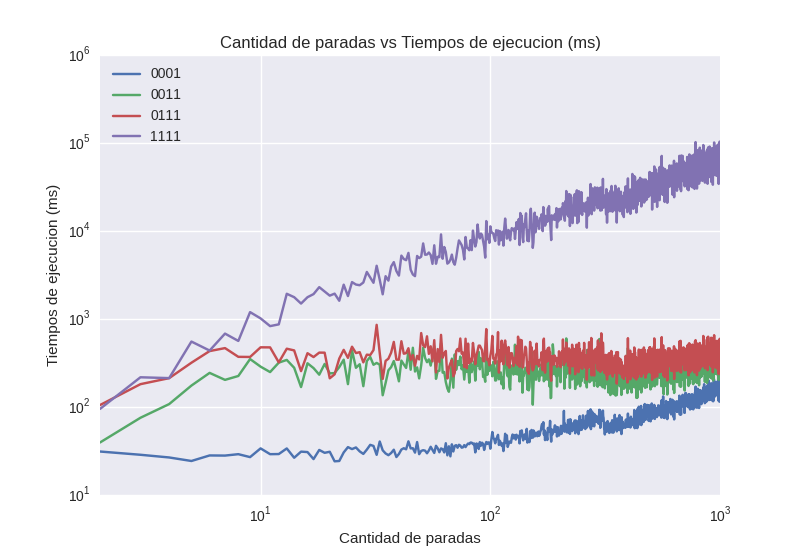
\includegraphics[width=\textwidth]{img/ejercicio3/exp1.png}
    \caption{Resultados del experimento 1.}
    \label{fig: ej3_exp1}
  \end{center}
\end{figure}

\par En la figura \ref{fig: ej3_exp1} podemos ver los resultados del experimento 1. Como esperábamos, vemos que las versiones con más vecindades conllevan mucho más tiempo de ejecución. Pero esto se verá reflejado en la calidad de la solución, ya que al buscar entre más vecindades creemos que tendrá más posibilidades de acercarte a la solución.

\par Para los casos con mayor cantidad de paradas notamos una diferencia muy grande. Inclusive, la versión $1111$ (con todas las vecindades) parece tomar una complejidad del orden cuadrático (lineal en el gráfico, porque los ejes están en escala logarítmica).





\subsubsection{Experimento 2: Cantidad de gimnasios vs Tiempos de ejecución}

\par En este caso, vamos a variar la cantidad de gimnasios y seguiremos midiendo los tiempos de ejecución de las distintas vecindades. Para esto, fijamos los parámetros \textit{cantidad de paradas = 100} y \textit{capacidad de la mochila = 5} y aumentaremos \textit{cantidad de gimnasios} desde 2 hasta 80.

\par Luego de haber visto los resultados del experimento anterior, esperamos aquí también que las versiones con más vecindades sufran mucho estos cálculos y esto se vea reflejado en los tiempos de ejecución. Queremos ver si se dan resultados similares al experimento anterior o si las complejidades cambian.

\begin{figure}[H]
  \begin{center}
    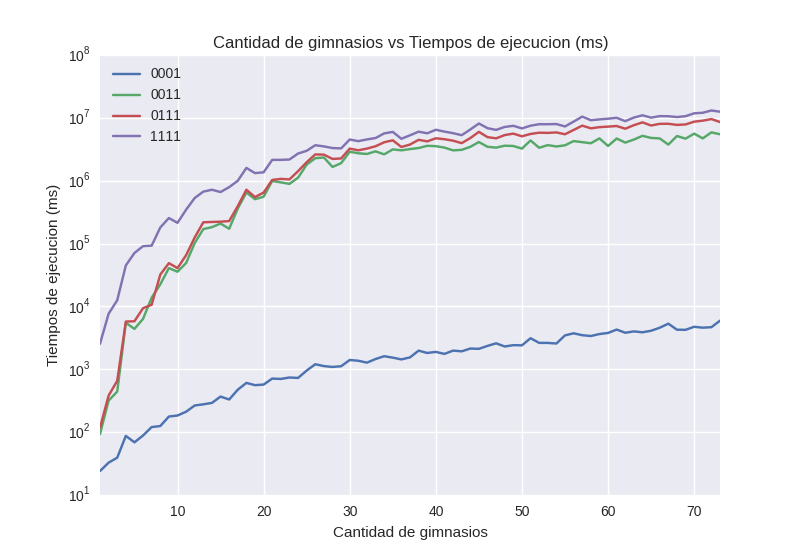
\includegraphics[width=\textwidth]{img/ejercicio3/exp2.png}
    \caption{Resultados del experimento 2.}
    \label{fig: ej3_exp2}
  \end{center}
\end{figure}

\par Con respecto al momento de ralizar la experimentación, debemos hacer un comentario. En un comienzo se había pensado en aumentar hasta la cantidad 300, pero se tuvo que limitar esta cantidad porque al ir aumentando los gimnasios se debe tomar \textit{cantidad de paradas} con un valor elevado y esto hizo que los tiempos de ejecución crecieran mucho más rápido. Luego de mucho tiempo de procesamiento, se debió frenar la experimentación en 80.

\par En la figura \ref{fig: ej3_exp2} podemos ver los resultados del experimento 2. Se nota claramente como la versión con solo un tipo de vecindad (0001) se ubica muy por debajo del resto. Lo que notamos también es que a partir de una cantidad elevada de gimnasios (aproximadamente 30) la diferencia entre las otras tres versiones se achica y se mantiene bastante estable. Esto creemos que es un punto a favor para utilizar la versión con más vecindades (1111), porque vemos que para casos más interesantes los tiempos de ejecución, con respecto a las versiones 0111 y 0011, no se diferencia tanto. Tendremos que tener en cuenta esto a la hora de comparar las versiones en función de la calidad de sus soluciones.



\subsubsection{Experimento 3: Calidad}

\par Luego de haber medido los tiempos de ejecución, creemos necesario comparar los resultados obtenidos entre las distintas versiones para poder luego, con los experimentos realizados, determinar qué versión será la definitiva.

\par Para comparar las soluciones que nos brinda cada versión correremos una serie de casos de distintos tipos y analizaremos los datos obtenidos. Estos casos van a ser generados de la siguiente forma:

\begin{itemize}
  \item para el parámetro \textit{cantidad de gimnasios} se toma un valor de manera aleatoria entre 1 y 10.
  \item para el parámetro \textit{cantidad de paradas} se toma un valor de manera aleatoria entre 1 y 10.
  \item para el parámetro \textit{capcidad de la mochila} se toma un valor de manera aleatoria entre 1 y 7.
\end{itemize}

\par Se generaron 100 casos. Algunos de los casos generados resultaron ser inválidos (sin solución), ya que no queríamos dejar afuera estos casos, aunque para algunos análisis se los va a dejar de lado.

\par Se corrieron estos casos en las 4 versiones y en el algoritmo exacto. A partir de ahora analizaremos los resultados obtenidos.

\medskip

\textbf{Análisis 1: Porcentaje de error}

\par Lo primero que queremos ver en los resultados de la experimentación es qué tan cerca de la solución exacta estuvo cada versión del programa. Para esto, realizamos un procentaje de error en cada caso de entrada. Por ejemplo, si la solución exacta era $10$ y el programa nos dió $9$, hay un 10\% de error. Luego sacamos un promedio del procentaje de error de todos los casos agrupado por versión del programa y obtuvimos los datos que vemos en el cuadro \ref{tab: ej3_exp3_an1_prom}.

\newcolumntype{C}[1]{>{\centering\let\newline\\\arraybackslash\hspace{0pt}}m{#1}}

\begin{table}[!htb]
  \caption{Porcentajes de error por versión del programa}
  \label{tab: ej3_exp3_an1_prom}
  \begin{subtable}{.5\linewidth}
    \caption{Todos los casos.}
    \label{tab: ej3_exp3_an1_prom_todos}
    \centering
    \begin{tabular}{|C{0.5cm}|C{2cm}|C{2cm}|}
      \hline
      {} & Versión del programa &  Porcentaje de error \\
      \hline
      0 &             '0001' &            69.13\\
      1 &             '0011' &            50.13\\
      2 &             '0111' &            34.45\\
      3 &             '1111' &            30.14\\
      \hline
    \end{tabular}
  \end{subtable}
  \begin{subtable}{.5\linewidth}
    \centering
    \caption{Casos con solución válida.}
    \label{tab: ej3_exp3_an1_prom_validados}
    \begin{tabular}{|C{0.5cm}|C{2cm}|C{2cm}|}
      \hline
      {} & Versión del programa &  Porcentaje de error \\
      \hline
      0 &             '0001' &            73.93\\
      1 &             '0011' &            53.61\\
      2 &             '0111' &            36.84\\
      3 &             '1111' &            32.23\\
      \hline
    \end{tabular}
  \end{subtable}
\end{table}

\par En ambos cuadros podemos ver que el procentaje de error va disminuyendo a medida que se aplican más tipos de vecindad. Esto era de esperarse. Pero lo que nos sorprende es la magnitud de las diferencias. Por ejemplo, en el cuadro \ref{tab: ej3_exp3_an1_prom_validados} vemos que la versión $0011$ tiene un procentaje de error del 50.47\%. Consideramos este valor como una aproximación muy burda de la solución, ya que estaría haciendo recorrer un 50\% más de distancia. En cambio las versiones $0111$ y $1111$ tiene un procentaje cercano al 30\%. Esta cota si nos parece un poco más acertada, pero queremos ver más en detalle cómo se distribuyen esos errores. Porque, por ejemplo, que el promedio de la versión $1111$ sea el 30.14\% nos da una idea, pero no sabemos si hay alguna solución muy lejana que nos esté influenciando mucho y tal vez separando un par de casos particulares podemos obtener un promedio mejor.

\par Para analizar mejor estos valores vamos a ver cómo se distribuyen estos porcentajes de error. Nos vamos a enfocar únicamente en los casos con solución válida.

\begin{figure}[H]
  \begin{center}
    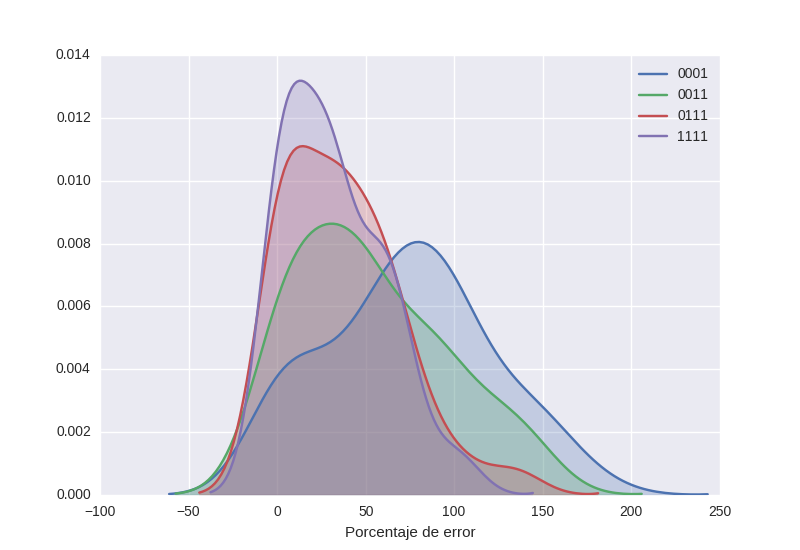
\includegraphics[width=\textwidth]{img/ejercicio3/exp3_distribuciones.png}
    \caption{Distribución de los porcentajes de error sobre casos con solución válida.}
    \label{fig: ej3_exp3_an1_distr_validados}
  \end{center}
\end{figure}

\par Podemos ver en la figura \ref{fig: ej3_exp3_an1_distr_validados} cómo los porcentajes de error obtenidos por la versión $1111$ se mantienen en un rango acotado, siendo el promedio un valor bastante representativo de los resultados en general. Esto nos indica que podemos acercanos en un 30\% a la solución exacta del problema con una probabilidad grande. Mientras que por ejemplo la versión $0111$ presenta una amplitud de porcentajes mayor, lo que nos indica que podemos obtener un resultado cercano al 30\%, pero que también tenemos una probabilidad (menor, pero no despreciable) de obtener un resultado que se diferencie en un 50\% y hasta 100\% de la solución exacta.



\subsubsection{Experimento 4: Cota del ciclo}

\par En este último experimento, queremos poner a prueba la cota máxima de iteraciones que le impusimos al ciclo del algoritmo. Hasta el momento solo la mencionamos. Por esto, queremos correr una cantidad importante de casos aleatorios para ver qué cantidad de veces ingresan al ciclo y analizar así si la cota impuesta es buena o si estamos perdiendo calidad saliendo antes del ciclo.

\par Para lleva a cabo el experimento, generamos una serie de casos random aumentando la cantidad de nodos desde 2 hasta 500. Para cada cantidad generamos varios casos. Luego, correremos estos casos sobre la versión $1111$ y contaremos la cantidad de veces que ingresa al ciclo.

\begin{figure}[H]
  \begin{center}
    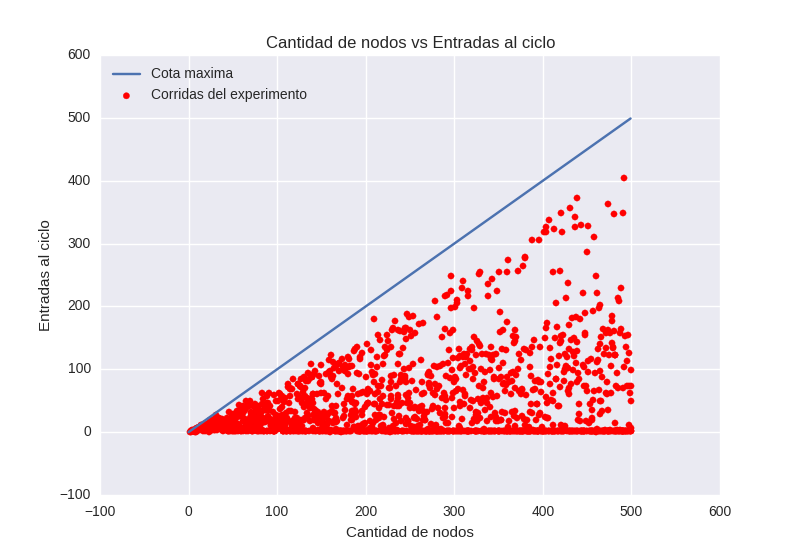
\includegraphics[width=\textwidth]{img/ejercicio3/exp4.png}
    \caption{Resultados del experimento 4.}
    \label{fig: ej3_exp4}
  \end{center}
\end{figure}

\par En la figura \ref{fig: ej3_exp4} podemos ver los resultados del experimento. La linea en azul indica la cota implementada, mientras que los puntos rojos son los datos obtenidos de las corridas. Notamos que la cantidad de entradas al ciclo se mantiene por debajo de la cota, lo que nos indica que la cota no nos está privando de mejores soluciones, sino que el algoritmo sale del ciclo (porque no logra mejorar la solución) antes de llegar a la cota. Solo en los casos con cantidad de nodos muy pequeña vemos que llega a la cota, pero a partir de aproximadamente 30 nodos la cota deja de influir.

\par Podemos concluir así que la cota tomada es buena y parece comportarse correctamente. No podemos asegurar que esto ocurra para todos los casos posibles, pero consideramos que la cota se comporta bien para una buena cantidad y vamos a dejarla.



\bigskip

\par Concluimos que la mejor versión es la que utiliza todas las vecindades ($1111$). A pesar de que nos hubiera gustado indagar más profundo en cuanto a la relación calidad-tiempo, creemos que los tiempos de ejecución no son tan elevados en los casos generales. En cuanto a calidad, nos quedamos claramente con las versiones $0111$ y $1111$. En cuanto a tiempos, vimos que para algunos casos había una gran diferencia y para otros no. Por esto nos quedamos con la versión que nos asegura mejora calidad y correremos los riesgos de tener casos con tiempos de ejecución elevados. más adelante (en el ejercicio 5) podremos ver si esta decisión fue acertada o si los tiempos de ejecución castigan a este algoritmo y no le permiten competir fuertemente con los otros algoritmos.

\newpage
\section{Ejercicio 4: Metaheurística}
Para mejorar la calidad de la soluci\'on dada por la heur\'istica de b\'usqueda local decidimos usar la metaheur\'istica GRASP (Greedy Randomized Adaptive Search Procedure). Esta metaheur\'istica consiste en generar varias soluciones iniciales (por ejemplo bas\'andose en una heur\'istica greedy) y luego mejorarlas con una b'usqueda local. \\
Nosotros proponemos como soluciones iniciales cuatro \emph{greedies}, cada uno con una condici\'on distinta de decisi\'on del pr\'oximo gimnasio:
\begin{itemize}
    \item El m\'as cercano.
    \item El m\'as lejano.
    \item El m\'as fuerte.
    \item El m\'as d\'ebil.
\end{itemize}

Para que el GRASP sea efectivo cada vez que se puede ir a un gimnasio se elige entre las $n/2$ mejores opciones siendo $n$ la cantidad total de gimnasios. En caso de que haya menos opciones se elegiran entre todos. La elecci\'on se realiza mediante un n\'umero generado pseudoaleatoriamente.

\subsection{Pseudoc\'odigo}

\SetAlgoLined
\SetKwProg{Fn}{Function}{:}{EndFunction}
\begin{algorithm}[H]
	\label{algo: ejercicio4_pseudocodigo}
	\Fn{GRASP}{
	    solucion
		
    	\BlankLine
		\For{desde 0 hasta la cantidad de pokeparadas}{
			\For{cada configuracion de goloso}{
			    solucionParcial $\gets$ calcularGoloso() \\
			    busquedalocal(solucionParcial)\\
			    \If{distancia(solucion)$>$ distancia(solucionParcial)}{
			        solucion $\gets$ solucionParcial
			    }
			}
        }
        return solucion
}
	\caption{Función que implementa la metaheur\'istica GRASP.}
\end{algorithm}


\SetAlgoLined
\SetKwProg{Fn}{Function}{:}{EndFunction}
\begin{algorithm}[H]
	\label{algo: ejercicio4_golosopseudocodigo}
	\Fn{Goloso aleatorio}{
	    \BlankLine
	    		
		\If{hay pokeparadas}{
		    visito el nodo más cercano al primer gimnasio
		}\Else{
		    visito el primer gimnasio
		}
    	\BlankLine
		\While{no haya recorrido todos los gimnasios}{
		    \If{hay gimnasios a los que pueda ir}{
		        ordeno la lista de gimnasios posibles por distancia al nodo actual o cantidad de pociones segun corresponda \\
		        genero un numero pseudoaleatorio entre 0 y la cantidad de gimnasios posibles exclusive \\
		        visito gimnasios\_posibles[random]
		    }\Else{
		        \If{hay pokeparadas sin visitar}{
		            visito la pokeparada más cercana al ultimo nodo visitado
		        }\Else{
		            \Return no existe solucion
		        }
		    }
		}
        \Return la lista con todos los nodos visitados
    }
	\caption{Función que implementa la creaci\'on de la soluci\'on inicial.}
\end{algorithm}


\subsection{Cota de complejidad}
Primero veamos que el goloso para generar la soluci\'on inicial cuesta $O(n^2+(mlog(m))^2))$ con $n$ la cantida de paradas y $m$ la cantidad de gimnasios. La guarda de la l\'inea 2 cuesta $O(1)$ ya que lo representamos con un vector a las pokeparadas. Cualquiera de las dos bifurcaciones cuesta $O(1)$ ya que se agrega un entero al final de una lista. Luego se realizamos un ciclo while, cuyo peor caso es recorrer todas las pokeparadas y, por supuesto, todos los gimnasios. La evaluaci\'on de la guarda cuesta $O(1)$ ya que utilizamos un contador de gimnasios visitados. Despu\'es, en la l\'inea 9 para verificar esa condici\'on recorremos todos los gimnasios y validamos que se cuente con las pociones suficientes para atacarlo y que no lo hayamos visitado a\'un, esto cuesta $O(m)$. La rama verdadera del if es $O(mlog(m))$ ya que ordenar cuesta $O(mlog(m))$ porque en peor caso tengo todos los gimnasios, generar el n\'umero pseudoaleatorio es $O(1)$ y agregar un entero a una lista tambi\'en. En cambio la rama falsa es $O(n)$ ya que se recorren todas las pokeparadas para encontrar la m\'as cercana (en caso de que hay alguna sin visitar). \\
Recapitulando en el ciclo while hay 2 casos, cuando se visita una pokeparada es $O(n)$ y cuando se visita un gimnasio es $O(mlog(m))$, dado que en peor caso nuestro ciclo se ejecuta $O(n+m)$ veces la complejidad total es $O(n^2+(mlog(m))^2))$.

Comencemos analizando el cuerpo del ciclo for de la l\'inea 4. El c\'alculo del goloso de la l\'inea 5 cuesta $O(n^2+(mlog(m))^2)$, la b\'usqueda local de la l\'inea 6 cuesta $O(max(n^4,m^4))$, la guarda de la l\'inea 6 se puede computar en $O(n+m)$ ya que calcular la distancia de un camino es $O(n+m)$ y luego se realiza una comparaci\'on de enteros. Por \'ultimo se copia un vector a otro que tambi\'en cuesta $O(n+m)$. En total el cuerpo de ese for cuesta $O(max(n^4,m^4))$ ya que s\'olo hay 4 configuraciones posibles para nuestro goloso. El ciclo for de la linea 3 hace que nuestro algoritmo tenga complejidad $O(max(n^5,m^5)$ ya que hay $O(n)$ paradas en total.

\subsection{Experimentaci\'on}

Para esta heur\'istica propusimos los siguientes experimentos:

\begin{itemize}

\item Paradas y Gimnasios: Si el enfoque est\'a en la cantidad de nodos se ve que el tiempo de ejecuci\'on pareciera tener una tendencia menor o igual a la complejidad teórica.

\begin{figure}[H]
	\begin{center}
		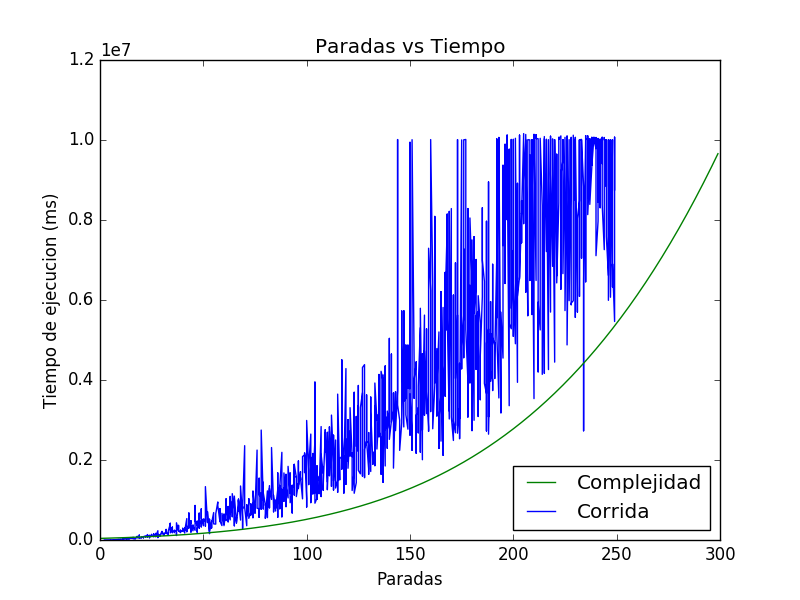
\includegraphics[width=0.7\textwidth]{img/ejercicio4/ParadasTiempos.png}
		\caption{}
		\label{fig: Paradas}
	\end{center}
\end{figure}
\begin{figure}[H]
	\begin{center}
		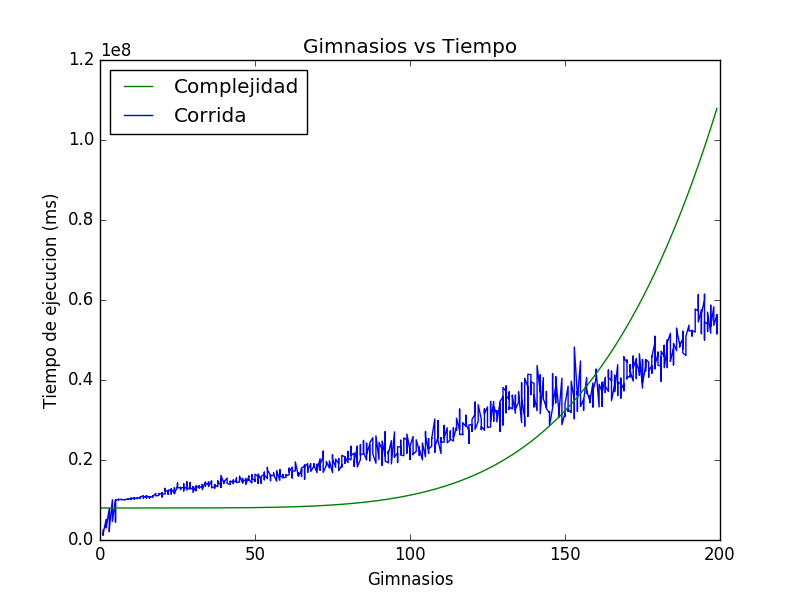
\includegraphics[width=0.7\textwidth]{img/ejercicio4/GimnasiosTiempos.png}
		\caption{}
		\label{fig: Gimnasios}
	\end{center}
\end{figure}


\item Gimnasios: 

Es obvio que si se aumenta la cantidad de gimnasios el tiempo de ejecuci\'on va a aumentar pero lo que queremos mostrar es que si se aumenta la cantidad de nodos obligatorios para el camino el tiempo de ejecuci\'on aumenta dado que a la fuerza tiene que construir un camino m\'as largo. Es importante aclarar que para este experimento tuvimos en cuenta que siempre haya alguna soluci\'on posible, sencillamente se fij\'o la cantidad de nodos totales en 20 y se vari\'o la cantidad de gimnasios. Los casos en los cuales no hay soluci\'on posible no son muy interesantes dado que los algoritmos golosos no iban a devolver una soluci\'on entonces las b\'usquedas locales no se iban a ejecutar.


\begin{figure}[H]
	\begin{center}
		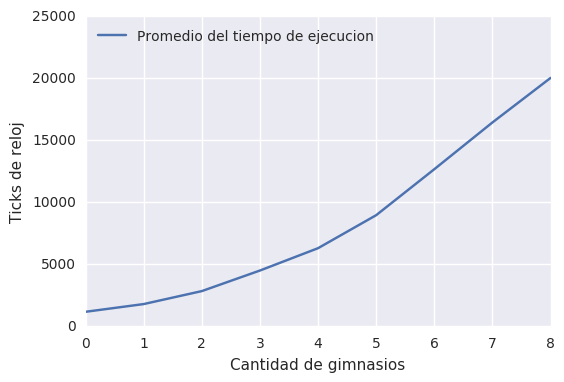
\includegraphics[width=0.7\textwidth]{img/ejercicio4/gimnasios.png}
		\caption{}
		\label{fig: ej4_gimnasios}
	\end{center}
\end{figure}

\item Capacidad de la mochila: 

\begin{figure}[H]
	\begin{center}
		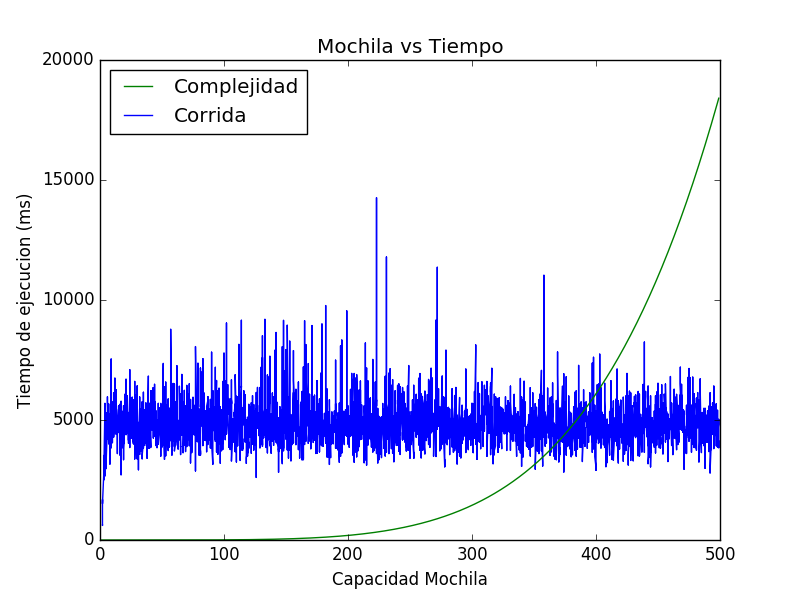
\includegraphics[width=0.7\textwidth]{img/ejercicio4/MochilaTiempos.png}
		\caption{}
		\label{fig: ej4_mochila}
	\end{center}
\end{figure}

En este gr\'afico podemos ver que aumentar la capacidad de la mochila no genera un aumento en el tiempo de ejecuci\'on, inclusive se aprecia que sigue la tendencia nula de una función constante . El rol de la capacidad de la mochila es m\'as que nada para decidir si hay una soluci\'on posible o no, aunque tambi\'en influye levente en la cantidad de pokeparadas visitadas en el camino.

\item Calidad: 

Vemos la diferencia absoluta entre la distancia exacta y la calculada con grasp variando la capacidad de la mochila y luego variando la cantidad de paradas:
\begin{figure}[H]
	\begin{center}
		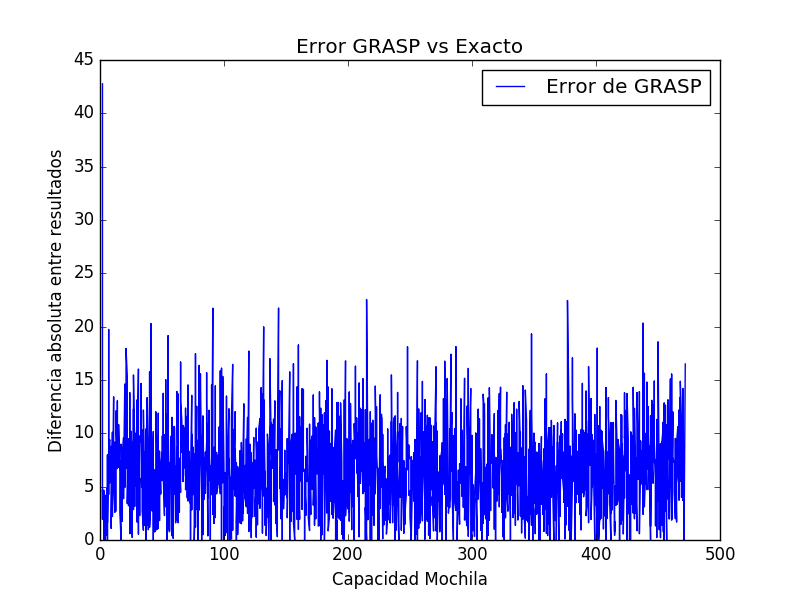
\includegraphics[width=0.7\textwidth]{img/ejercicio4/CalidadMochilas.png}
		\caption{}
		\label{fig: ej4_gimnasios}
	\end{center}
\end{figure}

\begin{figure}[H]
	\begin{center}
		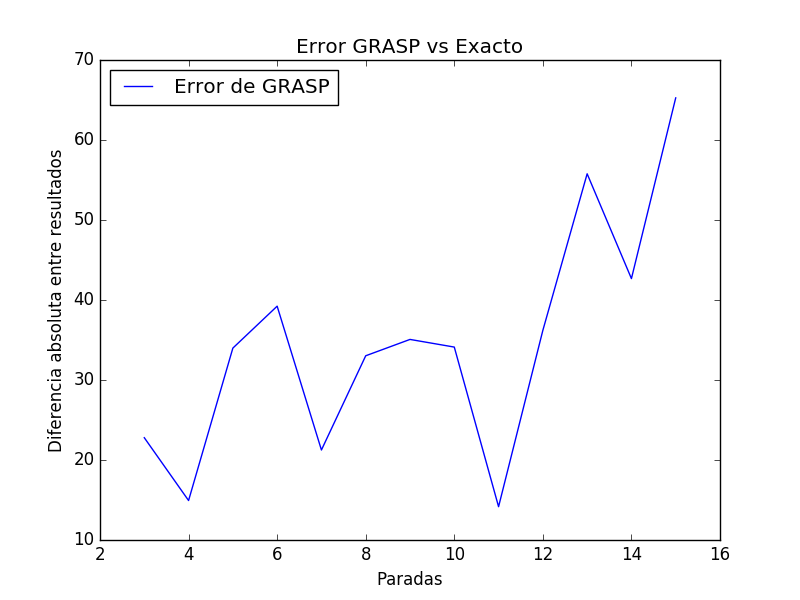
\includegraphics[width=0.7\textwidth]{img/ejercicio4/CalidadPokes.png}
		\caption{}
		\label{fig: ej4_mochila}
	\end{center}
\end{figure}

En el caso de variar la mochila, se ve como el error es constante sobre la capacidad de la mochila.\newline
En el segundo gráfico tenemos pocos nodos como para sacar una conclusión
\end{itemize}



\newpage
\section{Ejercicio 5: Comparación de Heurísticas}
\par En este último ejercicio vamos a poner a prueba las distintas heurísticas y metaheurísticas planteadas en los ejercicios previos con una serie de casos y compararemos su rendimiento y la calidad de la solución. La idea principal de esta sección es sacar conclusiones sobre en qué aspectos un algoritmo se desempeña y en qué aspectos no consideramos beneficioso utilizarlo.

\par Antes de comenzar, definiremos una numeración para los programas. Esto hará más fácil la explicación y la referencia a cada programa.

\begin{itemize}
	\item \textbf{Programa 1}: Programa visto en el ejercicio 1, basando en un algoritmo de backtracking. Genera una solución exacta.
	\item \textbf{Programa 2}: Programa visto en el ejercicio 2, implementación de un algoritmo basado en una heurística golosa.
	\item \textbf{Programa 3}: Programa visto en el ejercicio 3, implementación de un algoritmo basado en una heurística de búsqueda local.
	\item \textbf{Programa 4}: Programa visto en el ejercicio 4, implementación de un algoritmo basado en una metheurística que busca mejorar las soluciones dadas por la heurística de búsqueda local (programa 3).
\end{itemize}

\subsection{Generación de casos}

\par Para generar los casos utilizamos un script que recibe la cantidad de nodos del tipo gimnasio, la cantidad de nodos del tipo parada y la capacidad de la mochila. Luego, en base a estos datos, genera un caso de entrada al problema. Tanto la ubicación de los nodos como las pociones necesarias para matar a un gimnasio son generados de forma aleatoria dentro de un rango seteado manualmente.

\par Para el experimento se generaron casos que van desde 2 nodos hasta 3000. Se fué aumentando esta cantidad de nodos dependiendo de la cantidad actual, para generar más esparcimiento con cantidades más grandes. Por ejemplo, de 5 nodos se pasó a 6, pero de 155 nodos se pasó a 159, mientras que de 1402 se pasó a 1438.

\subsection{Ejecución del experimento}

\par Debido a los tiempos de ejecución de cada programa, se decidió establecer rangos en los cuales se correrán cada programa. Por ejemplo, se sabe que el programa 1 tiene una complejidad elevada y por eso se diseñan heurísticas que den soluciones cercanas en menos tiempo. Por esto el programa será ejecutado para casos de entrada con menor cantidad de nodos que el resto.

\medskip

\par En base a esto, en el cuadro \ref{tab: ej5_rangos} se encuentran definidos los rangos y qué programas serán ejecutados en cada uno. Todos los rangos comienzan con un valor de 2 nodos, y luego es extienden hasta su valor máximo (especificado en el cuadro).

\newcolumntype{C}[1]{>{\centering\let\newline\\\arraybackslash\hspace{0pt}}m{#1}}

\begin{table}[h]
	\centering
	\begin{tabular}{|C{1.2cm}|C{2cm}|C{2.3cm}|C{2.3cm}|C{2.3cm}|C{2.3cm}|C{2.3cm}|}
		\hline
		\textbf{Rango} & \textbf{\#Nodos máximo} & \textbf{Programa 1} & \textbf{Programa 2} & \textbf{Programa 3} & \textbf{Programa 4} \\ \hline
		\textbf{1} & 20 & \cellcolor{green}SI & \cellcolor{green}SI & \cellcolor{green}SI & \cellcolor{green}SI \\ \hline
		\textbf{2} & 200 & \cellcolor{gray}NO & \cellcolor{green}SI & \cellcolor{green}SI & \cellcolor{green}SI \\ \hline
		\textbf{3} & 1000 & \cellcolor{gray}NO & \cellcolor{green}SI & \cellcolor{green}SI & \cellcolor{gray}NO \\ \hline
	\end{tabular}
	\caption{Rangos: cantidad de nodos y programas que se ejecutan.}
	\label{tab: ej5_rangos}
\end{table}

\par Cabe aclarar que el rango de un algoritmo no indica que no consideremos utilizarlo por fuera de él. Dependiendo el caso, puede ser bueno correr un programa, por ejemplo, 1 hora. Mientras que para una experimentación, correr un caso de 1 hora no es viable.



\par A continuación analizaremos los resultados obtenidos. Para esto, dividiremos los análisis en los distintos rangos.

\subsection{Análisis 1: Tiempos de ejecución en el rango 1}

\par Como mencionamos previamente, correremos todos los algoritmos con casos de entrada generados aleatoriamente. Comenzaremos con \textit{cantidad de nodos} = 2 y aumentaremos este parámetro hasta 20. Luego analizaremos los resultados obtenidos de las mediciones de tiempo y compararemos los distintos programas.

\par Esperamos que el programa 1 (algoritmo de backtracking) se posicione muy por encima del resto. Lo que si nos interesa ver, es qué tanto se diferencia de los demás. Esta diferencia será interesante tenerla en cuenta al momento de comparar calidades de la solución de cada heurística.

\begin{figure}[H]
  \begin{center}
    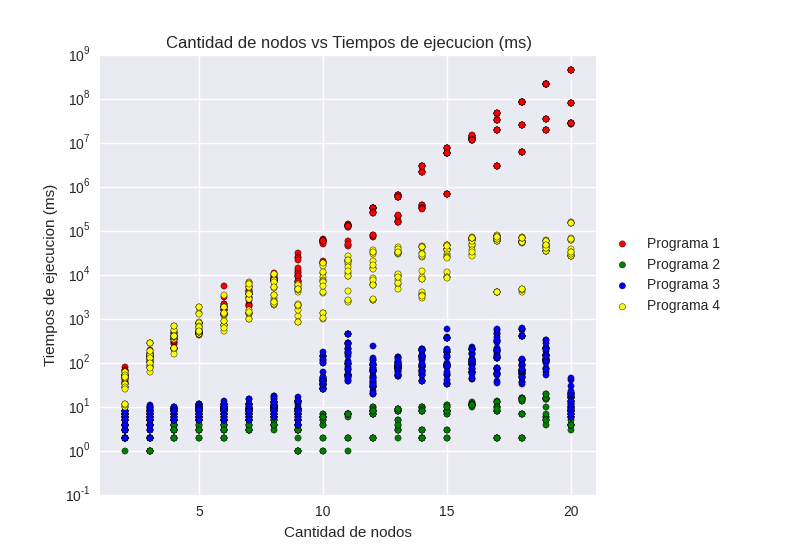
\includegraphics[width=\textwidth]{img/ejercicio5/tiempos_r1.png}
    \caption{Tiempos de ejecución en el rango 1. Programas 1, 2, 3 y 4}
    \label{fig: ej5_tiempos_r1}
  \end{center}
\end{figure}

\par En la figura \ref{fig: ej5_tiempos_r1} podemos ver los resultados del experimento. Notamos cláramente como el programa 1 se posiciona por encima del resto. Vemos también como el programa 4, en un primer momento mantiene tiempos similares. Esto se lo adjudicamos al hecho de que, al ser una cantidad muy reducida de nodos, calcular las vecindades para distintos resultados de una heurística golosa puede ser igual a pasar por las distintas soluciones válidas del problema (que es justamente lo que realiza el programa 1). Luego, a partir de los 10 nodos, se ve como calcular las vecindades deja de ser tan significativo.

\par A pesar de que el programa 4 se basa en una heurística de búsqueda local, al igual que el programa 3, la diferencia es que el primero realiza una cantidad grande de soluciones golososas y esto le da una cantidad grande de tipos de solucones válidas. Al buscar las vecindades de estos diversos tipos, se recorren más instancias.

\par Por su parte los programas 2 y 3 en ningún momento manejan tiempos cercanos al programa 1. Este también es un factor importante para tener en cuenta al comparar la calidad de las soluciones. Igualmente, a continuación veremos si esto se mantiene para otros rangos.

\subsection{Análisis 2: Tiempos de ejecución en el rango 2}

\par En este caso, correremos los programas 2, 3 y 4. Partimos de \textit{cantidad de nodos} = 2 y llegaremos hasta 200. Mediremos los tiempos de ejecución y luego analizaremos los resultados obtenidos.

\par Esperamos ver que el programa 4 tenga tiempos de ejecución mucho mayores a los otros dos. También queremos ver si entre los programas 2 y 3 comienzan a marcarse diferencias, ya que en el rango 1 vimos que comenzaban a separarse, pero no definidamente.

\begin{figure}[H]
  \begin{center}
    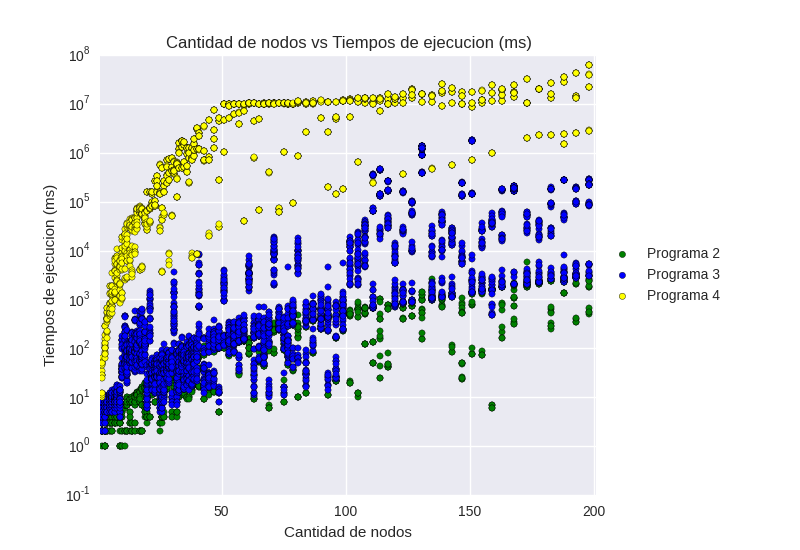
\includegraphics[width=\textwidth]{img/ejercicio5/tiempos_r2.png}
    \caption{Tiempos de ejecución en el rango 2. Programas 2, 3 y 4}
    \label{fig: ej5_tiempos_r2}
  \end{center}
\end{figure}

\par En la figura \ref{fig: ej5_tiempos_r2} podemos ver los resultados del experimento. Notamos como el programa 4 se desprende del resto y se mantiene en tiempos de ejecución muy por encima del resto. Pero un detalle interesante que notamos, es como a partir de los 50 nodos el tiempo se aplana bastante y deja de crecer de la manera en que venía haciéndolo. Esto se debe a que comienza a influir la cota de cantidad de ticks que se pone. A partir de una cierta cantidad de ticks de ejecución, el programa comienza a saltear nodos de inicio y termina más rápido la ejecución. Esto puede afectar mucho la calidad, pero de alguna forma debemos acotar los tiempos de ejecución.

\par Podemos ver como el programa 3 tiene algunos casos con tiempos cercanos al programa 2, mientras que en algunos casos estos tiempos se elevan. Esto se debe a que la heurística de búsqueda local depende mucho del caso de entrada. Si el caso de entrada puede aproximarse bien por la heurística golosa, luego se harán pocas mejoras y se obtendrá un tiempo cercano al programa 2 (que se basa justamente en una heurística golosa). También hay que tener en cuenta que entre los casos de experimentación hay casos inválidos. Esto hace que el programa 3, al llamar a la heurística golosa verifique que no le devolvió solución y no realice cambios (evitando así calcular las vecindades).

\subsection{Análisis 3: Tiempos de ejecución en el rango 3}

\par Para este último rango vamos a correr los programas 2 y 3. Partiremos de 2 nodos y llegaremos hasta 1000. Ahora sí vamos a exigir al programa 3, y esperamos que sus tiempos de ejecución se marquen muy por encima del programa 2. Pero nos interesa en particular ver qué tanta diferencia se ve entre ellos.

\begin{figure}[H]
  \begin{center}
    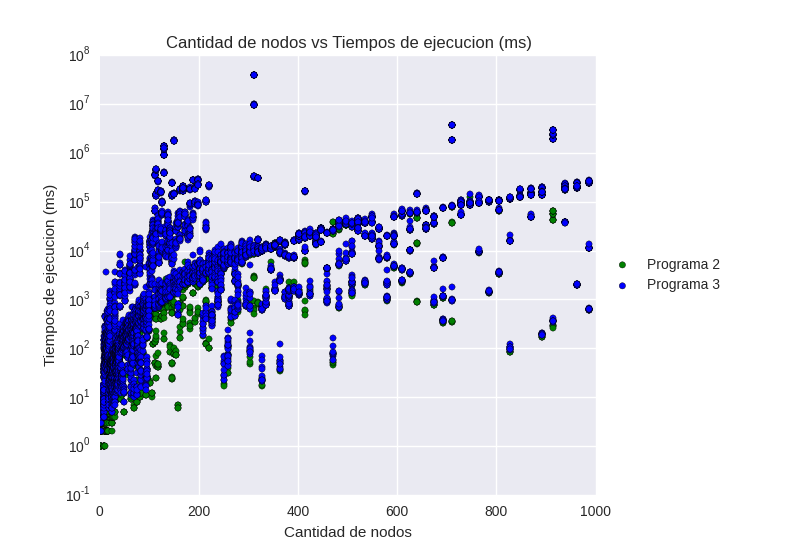
\includegraphics[width=\textwidth]{img/ejercicio5/tiempos_r3.png}
    \caption{Tiempos de ejecución en el rango 3. Programas 2 y 3}
    \label{fig: ej5_tiempos_r3}
  \end{center}
\end{figure}

\par En la figura \ref{fig: ej5_tiempos_r3} podemos ver los resultados del experiento. Lo primero que notamos es que no se ve tanta diferencia entre los programas como esperábamos. Si se ve que el programa 3 toma valores más dispersos en un primer momento, hasta aproximadamente 200 nodos. A partir de ahí, los valores del programa 3 se ven bastante cercanos a los del programa 2. Creemos que hay dos factores que pudieron ser muy importantes para que se de esto:

\begin{itemize}
	\item que el generador se haya mantenido en casos parecidos y por eso tengamos tiempos similares;
	\item que la heurística golosa haya sido bastante acertada y no se hagan muchos cambios en la búsqueda local.
\end{itemize}

\par Pero en principio, no notamos tanta diferencia entre los problemas. Tendremos que tener en cuenta esto a la hora de comparar calidad de las soluciones.


\subsection{Calidad de las soluciones}

\par Luego de haber analizado los tiempos de ejecución de los programas, vamos a ver la calidad de las soluciones comparándolas con el programa 1 (solución exacta). Para esto vamos a centrarnos en los resultados obtenidos en el rango 1, ya que era el único rango en el cuál corrimos el programa 1.

\par Vamos a presentar los resultados desde distintos enfoques para observar distintos detalles que creamos interesantes.

\subsubsection{Análisis 4: Porcentajes de error}

\par Lo primero que vamos a hacer es ver los porcentajes de error de cada caso, sacar promedios y ver cómo es su distribución.

\begin{table}[!htb]
	\caption{Porcentajes de error por programa}
	\label{tab: ej5_an4_porc_error}
	\begin{subtable}{.5\linewidth}
		\caption{Todos los casos.}
		\label{tab: ej5_an4_porc_error_todos}
		\centering
		\begin{tabular}{|C{2cm}|C{3.5cm}|}
			\hline
			Programa & Promedio de error \\
			\hline
			2 & 46.88 \% \\
			3 & 45.35 \% \\
			4 & 12.06 \% \\
			\hline
		\end{tabular}
	\end{subtable}
	\begin{subtable}{.5\linewidth}
		\centering
		\caption{Casos con solución válida.}
		\label{tab: ej5_an4_porc_error_validos}
		\begin{tabular}{|C{2cm}|C{3.5cm}|}
			\hline
			Programa & Promedio de error \\
			\hline
			2 & 48.14 \% \\
			3 & 46.58 \% \\
			4 & 12.38 \% \\
			\hline
		\end{tabular}
	\end{subtable}
\end{table}

\par En el cuadro \ref{tab: ej5_an4_porc_error} podemos ver los promedios de los porcentajes de error de cada programa. En los cuadro \ref{tab: ej5_an4_porc_error_validos} se encuentran diferenciados los casos válidos. Podemos ver que el programa 4 saca una gran diferencia en cuanto a calidad. Pasar de un error del 45\% a un error del 12\% es un cambio importante. Esto es un factor para contrastar con los resultados obtenidos en las mediciones de tiempos, donde el programa 4 marcó tiempos de ejecución notoriamente mayores a los de los programas 2 y 3.

\par Para ver más en detalle estos valores, en la figura \ref{fig: ej5_calidad_distr_porc} podemos ver la distribución de estos porcentajes. Viendo este gráfico reafirmamos la ventaja, en cuanto a calidad, del programa 4 por sobre el resto. Podemos ver que la mayor parte de sus porcentajes se encuentran muy cerca del cero, mientras que en los otros programas los porcentajes de error se distribuyen bastante más, posicionándose principalmente cerca del 50\%.

\begin{figure}[H]
  \begin{center}
    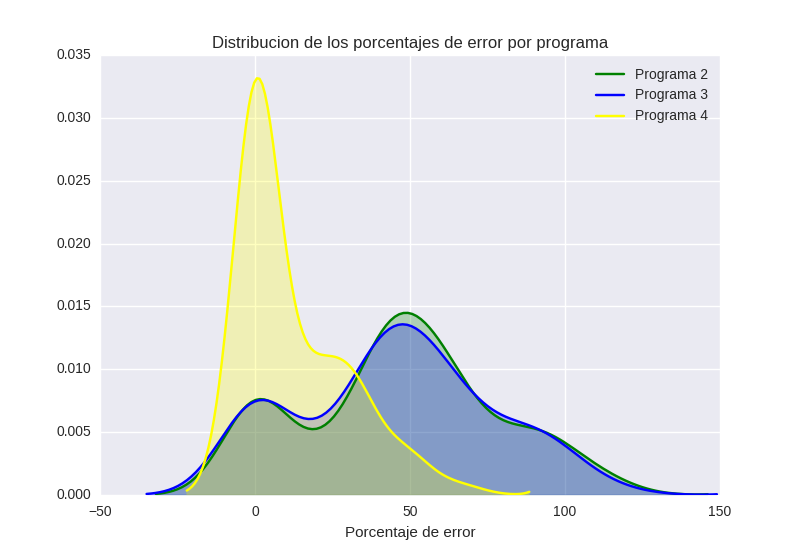
\includegraphics[width=\textwidth]{img/ejercicio5/calidad_distribuciones_error.png}
    \caption{Distribución de porcentajes de error por programa.}
    \label{fig: ej5_calidad_distr_porc}
  \end{center}
\end{figure}

\subsubsection{Análisis 5: Relación Tiempos-Calidad}

\par Luego de haber analizado la calidad de las soluciones brindadas por cada programa, nos vemos en la obligación de contrastar estos datos con los datos obtenidos en los experimentos previos. Para eso, vamos a definir una relación entre el tiempo de ejecución y el error de la solución final y veremos qué podemos ver a partir de esto.

\begin{figure}[H]
  \begin{center}
    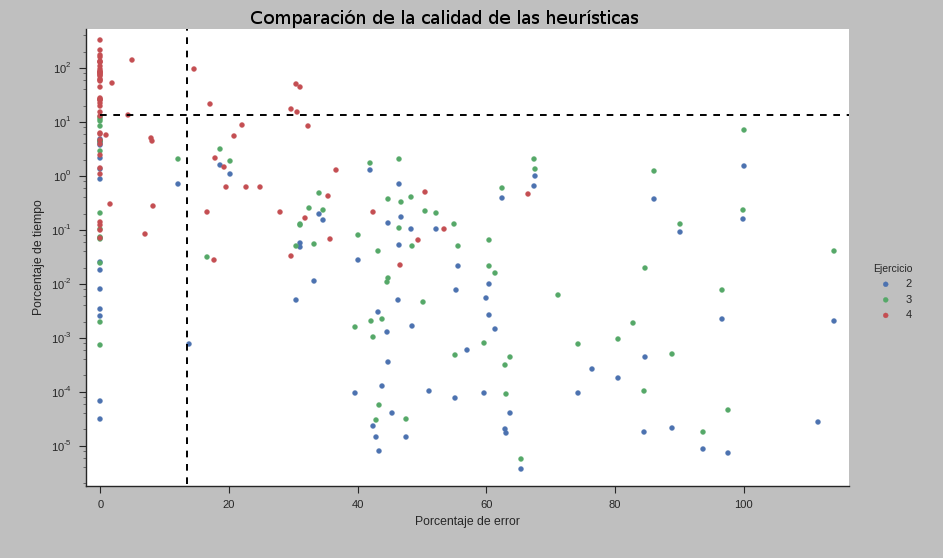
\includegraphics[width=\textwidth]{img/ejercicio5/relacion_tiempo_calidad.png}
    \caption{Gr\'afico que muestra la relaci\'on entre calidad y tiempo.}
    \label{fig: ej5_relacion_tiempo_calidad}
  \end{center}
\end{figure}
En la figura de arriba la l\'inea punteada vertical representa la media de los tiempos de nuestros experimentos mientras que la l\'inea punteada horizontal muestra la media de los errores con respecto a la soluci\'on exacta.
En la figura se puede ver que en el cuadrante que est\'a a la izquierda de la media de error y por encima de la media de tiempos predomina el GRASP, lo cual quiere decir que si uno cuenta con mucho tiempo y quiere una muy buena soluci\'on puede usar esa heur\'istica. En el cuadrante inferior derecho predominan el algoritmo goloso y la b\'usqueda local. ESto nos quiere decir que son soluciones econ\'omicas en cuanto a tiempo pero no muy buenas en cuanto a la calidad de la soluci\'on. En el cuadrante que se encuentra a la izquierda de la media de error y debajo de la media de tiempos predomina (pero no en demas\'ia) el GRASP. En el cuadrante restante hay algunos casos de GRASP pero son outliers.\\
La conclusi\'on que podemos sacar de este gr\'afico es que si se prefiere que la soluci\'on sea buena requiere mucho tiempo de procesamiento, en cambio si se necesita una soluci\'on r\'apida pero sin importar cuanto difiere de la \'optima se pueden usar las otras dos heur\'isticas.

\newpage
\section{Anexo con el código}
\subsection{Estructura básica y funciones auxiliares}
\label{sec: anexo_ejercicio}
\par Aquí se define la clase \textbf{Ejercicio}, la cual continene las estructuras utilizadas para almacenar el grafo. También recibe la entrada y la almacena en la estructura. Y tiene funciones que son utilizadas en los distintos ejercicios.

\begin{lstlisting}
class ejercicio {
protected:
  double distanciaMinima;
  vector<int> solucion;
  vector<tuple<int,int,int>> gimnasios;
  vector<tuple<int,int>> pokeparadas;
  vector<vector<double>> distancias;
  int mochila;
  int pocionesActuales;
  bool entrada_invalida = false;


public:
  //-------------------------------------------------------------------------------------------
  //----- CONSTRUCTOR: Recibe los datos de entrada y llena las estructuras
  //-------------------------------------------------------------------------------------------
  ejercicio (){
    // parseo
    int n, m; // mochila = k
    cin >> n >> m >> mochila;

    int posx, posy, pociones;

    //--vamos a calcular la minima cantidad de pociones necesarias para matar a todos los gimnasios
    int min_pociones_necesarias = 0;

    for (size_t i = 0; i < n; i++) {
      cin >> posx >> posy >> pociones;
      //--acumula la cantidad de pociones necesarias para matar a todos los gimnasios
      min_pociones_necesarias += pociones;
      //--si se necesitan mas pociones de las que entran en la mochila => no hay solucion
      if (pociones > mochila) {
        entrada_invalida = true;
      }
      gimnasios.push_back(make_tuple(posx,posy,pociones));
    }

    for (size_t i = 0; i < m; i++) {
      cin >> posx >> posy;
      pokeparadas.push_back(make_tuple(posx,posy));
    }

    for (size_t i = 0; i < n+m; i++) {
      vector<double> dummy;
      distancias.push_back(dummy);
      for (size_t j = 0; j < n+m; j++) {
        int difX = 0;
        int difY = 0;
        if(i<n){ // el i es un gimnasio o una pokeparada?
          difX = get<0>(gimnasios[i]);
          difY = get<1>(gimnasios[i]);
        }else{
          difX = get<0>(pokeparadas[i-n]);
          difY = get<1>(pokeparadas[i-n]);
        }
        if(j<n){
          difX -= get<0>(gimnasios[j]);
          difY -= get<1>(gimnasios[j]);
        }else{
          difX -= get<0>(pokeparadas[j-n]);
          difY -= get<1>(pokeparadas[j-n]);
        }
        distancias[i].push_back(sqrt(pow(difX,2)+pow(difY,2)));
      }
    }

    pocionesActuales = 0;
    distanciaMinima = -1;

    //-- si no alcanzan las pokeparadas para juntar las pociones necesarias para matar a todos => no hay solucion
    if (min_pociones_necesarias > pokeparadas.size()*3) {
      entrada_invalida = true;
    }
  }


  //-------------------------------------------------------------------------------------------
  //----- IMPLEMENTACIONES DE ALGORITMOS GOLOSOS
  //-------------------------------------------------------------------------------------------

  //--GOLOSO BASICO:
  //--Trata de ir primero a los nodos mas cercanos. Sino va a una parada cercana.
  void golosoDeterministico(){
    // este goloso agarra el gimnasio mas cercano que puede matar
    int cant_gimnasios = gimnasios.size();
    int cant_poke = pokeparadas.size();
    int total = cant_poke+cant_gimnasios; // n+m

    // agarro el primer gimnasio y me voy a la poke parada mas cercana para arrancar
    int pokeCercano = pokeparadaMasCercana(0);

    pocionesActuales = sumaSaturada(pocionesActuales, 3);
    int gimnasios_recorridos = 0;
    int nodoActual = pokeCercano+cant_gimnasios;
    solucion.push_back(nodoActual+1);

    while (gimnasios_recorridos < cant_gimnasios) {
      int gimnasiocercano = -1;
      int distGim = -1;
      for (size_t i = 0; i < cant_gimnasios; i++) { // busco el mas cercano que puedo matar
        if ((distGim > distancias[i][nodoActual] || distGim == -1)// la distancia es menor
          && pocionesActuales >= get<2>(gimnasios[i]) // y me alcanzan las pociones
          && !yaLoRecorri(i)) // y no recorri este gimnasio
        {
          distGim = distancias[i][nodoActual];
          gimnasiocercano = i;
        }
      }
      if(gimnasiocercano == -1){ // no encontre gimnasio para matar, busco una pokeparada cerca
        pokeCercano = pokeparadaMasCercana(nodoActual);
        if (pokeCercano < 0) { // no quedan paradas => no puedo matar los gimnasios restantes
          break;
        } else {
          pocionesActuales = sumaSaturada(pocionesActuales,3);
          nodoActual = pokeCercano+cant_gimnasios;
        }
      } else { // mato el gimnasio!
        ++gimnasios_recorridos;
        nodoActual = gimnasiocercano;
        pocionesActuales -= get<2>(gimnasios[nodoActual]);
      }
      solucion.push_back(nodoActual+1);
    }

    if (gimnasios_recorridos < cant_gimnasios) {
      //-distancia invalida
      distanciaMinima = -1;
    } else {
      //-distancia
      distanciaMinima = 0;
      for(int i = 0; i < solucion.size()-1; ++i){
        distanciaMinima += distancias[solucion[i]-1][solucion[i+1]-1];
      }
    }

    return;
  }

  //--GOLOSO RANDOM:
  //--Recibe los siguientes parametros:
  //----nodo_inicial -> si quiere arrancar por una parada en particular
  //----orden_preferencia:
  //------0 va al mas cercano primero
  //------1 va al mas lejano primero
  //------2 va al que mas pociones necesite para matar
  //------3 va al que menos pociones necesite para matar
  //----cant_random -> la cantidad de nodos entre los que se va a tomar un random
  void calculaGoloso(int nodo_inicial = -1, int orden_preferencia = 0, int cant_random = 1) {

    int cant_gimnasios = gimnasios.size();
    int cant_poke = pokeparadas.size();
    int total = cant_poke+cant_gimnasios; // n+m

    int pocionesAct = 3;
    int gimnasios_recorridos = 0;

    int nodoActual = nodo_inicial;
    int pokeCercano;

    //--si no se paso un nodo de inicio como parametro
    if (nodo_inicial < 0) {
      // agarro una parada random
      if (cant_poke == 0) {
        nodoActual = 0;
        ++gimnasios_recorridos;
      } else {
        nodoActual = cant_gimnasios + rand() % cant_poke;
        pocionesAct = sumaSaturada(pocionesAct,3);
      }
    }
    solucion.clear();
    solucion.push_back(nodoActual + 1);

    while (gimnasios_recorridos < cant_gimnasios) {
      vector<tuple<int,float,int>> gimnasios_posibles; // vector<id,distancia,pociones>
      int gimnasiocercano = -1;
      for (size_t i = 0; i < cant_gimnasios; i++) { // busco los gimnasios que puedo matar
        if (pocionesAct >= get<2>(gimnasios[i]) // y me alcanzan las pociones
          && !yaLoRecorri(i)) // y no recorri este gimnasio
        {
            gimnasios_posibles.push_back(make_tuple(i,distancias[i][nodoActual],get<2>(gimnasios[i])));
        }
      }
      if(gimnasios_posibles.size() != 0){

        // actualizo cant random para que no haga randomen un cjto mayor
        int tope_random = cant_random > gimnasios_posibles.size() ? gimnasios_posibles.size() : cant_random;
        int random = rand()%tope_random;
        switch (orden_preferencia) {
          case 0:
            // busco los mas cercanos que pueda matar
            sort(gimnasios_posibles.begin(), gimnasios_posibles.end(), [](const tuple<int,float,int>& a,
            const tuple<int,float,int>& b) -> bool
            {
              return std::get<1>(a) > std::get<1>(b);
            });
            gimnasiocercano = get<0>(gimnasios_posibles[random]);
            break;

          case 1:
            // busco los mas lejanos que pueda matar
            sort(gimnasios_posibles.begin(), gimnasios_posibles.end(), [](const tuple<int,float,int>& a,
            const tuple<int,float,int>& b) -> bool
            {
              return std::get<1>(a) > std::get<1>(b);
            });
            gimnasiocercano = get<0>(gimnasios_posibles[gimnasios_posibles.size()-1-random]);
            break;

          case 2:
            // busco los que mas pociones necesite para matar y que pueda matar
            sort(gimnasios_posibles.begin(), gimnasios_posibles.end(), [](const tuple<int,float,int>& a,
            const tuple<int,float,int>& b) -> bool
            {
              return std::get<2>(a) > std::get<2>(b);
            });
            gimnasiocercano = get<0>(gimnasios_posibles[random]);
            break;

          case 3:
            // busco los que menos pociones necesite para matar y que pueda matar
            sort(gimnasios_posibles.begin(), gimnasios_posibles.end(), [](const tuple<int,float,int>& a,
            const tuple<int,float,int>& b) -> bool
            {
              return std::get<2>(a) > std::get<2>(b);
            });
            gimnasiocercano = get<0>(gimnasios_posibles[gimnasios_posibles.size()-1-random]);
            break;
        }
      }
      if (gimnasiocercano == -1) { // no encontre gimnasio para matar, busco una pokeparada cerca
        pokeCercano = pokeparadaMasCercana(nodoActual);
        if (pokeCercano < 0) { // no quedan paradas => no puedo matar los gimnasios restantes
          break;
        } else {
          pocionesAct = sumaSaturada(pocionesAct,3);
          nodoActual = pokeCercano+cant_gimnasios;
        }
      } else { // mato el gimnasio!
        ++gimnasios_recorridos;
        nodoActual = gimnasiocercano;
        pocionesAct -= get<2>(gimnasios[nodoActual]);
      }
      solucion.push_back(nodoActual+1);
    }

    //--si faltaron gimnasios por recorrer
    if (gimnasios_recorridos < cant_gimnasios) {
      //-distancia invalida
      distanciaMinima = -1;
    } else {
      //-distancia
      distanciaMinima = 0;
      for(int i = 0; i < solucion.size()-1; ++i){
        distanciaMinima += distancias[solucion[i]-1][solucion[i+1]-1];
      }
    }

    return;
  }


  //-------------------------------------------------------------------------------------------
  //----- IMPLEMENTACION DE BUSQUEDA LOCAL
  //-------------------------------------------------------------------------------------------

  //--Recibe el parametro:
  //----codigo_vecindades -> binario indicando cuales vecindades que se quieren usar y cuales no
  void busquedaLocal(string codigo_vecindades = "1111") {
    //--se usa esta variable para ver si se mejoro al solucion en el ultima iteracion
    bool cambio = true;

    int cant_nodos = gimnasios.size() + pokeparadas.size();
    int repeticiones = 0;

    //--mientras se mejore
    while(cambio && repeticiones < cant_nodos){

      cambio = false;

      vector<vector<int> > vecindad;

      //--pide las vecindades de la solucion actual
      for (int i = 0; i < 3; i++) {

        //--si la funcion de vecindad i esta marcada para ser usada
        if (codigo_vecindades[i] == '1') {

          vector<vector<int> > vecindad_nueva;

          //--llama a cada vecindad distinta
          switch (i) {

            case 0:
              //--cambia una parada del camino por una de afuera
              vecindad_nueva = vecinosConLosDeAfuera();
              break;

            case 1:
              //--cambia entre dos nodos adyacentes del camino (sin importar el tipo)
              vecindad_nueva = vecinosConLosAdyacentes();
              break;

            case 2:
              //--cambia entre dos paradas del camino
              vecindad_nueva = vecinosConLosDeAdentro();
              break;

            case 3:
              //--cambia entre dos gimnasios del camino
              vecindad_nueva = vecinosConLosGim();
              break;

          }

          //--si se tiene una nueva vecindad
          if (vecindad_nueva.size() > 0) {
            //--se agregan estos vecinos al final
            vecindad.insert(vecindad.begin(), vecindad_nueva.begin(), vecindad_nueva.end());
          }

        }

      }

      //--si la vecindad no esta vacia
      if(vecindad.size() > 0) {

        //--busca el mejor vecino
        vector<int> mejor_vecino = minimoVecino(vecindad);

        double dist_mejor_vecino = calcularDistancia(mejor_vecino);
        double dist_solucion = calcularDistancia(solucion);

        //--si el vecino es mejor que la solucion actual
        if (dist_mejor_vecino < dist_solucion) {

          //--cambia la solucion
          cambio = true;

          solucion = mejor_vecino;
          distanciaMinima = dist_mejor_vecino;

        }
      }

      //--aumenta el contador de repeticiones
      repeticiones++;
    }

    return;
  }



  //-------------------------------------------------------------------------------------------
  //----- IMPLEMENTACION DE VECINDADES
  //-------------------------------------------------------------------------------------------

  //--Vecindad 1: cambia paradas que esten en el camino por paradas que no esten en el camino
  vector <vector<int>> vecinosConLosDeAfuera() {
    int pokeNueva = 0;
    int pokeVieja = 0;
    vector<vector<int>> resultado;
    vector<int> solucionAMejorar = solucion;
    vector<tuple<int,int> > pokeswaps = pokeparadas;
    for( int i = 0; i< solucionAMejorar.size(); i++) {
      if (esPokeParada(solucionAMejorar[i])) {
        for (int j = 0; j < pokeswaps.size(); j ++) {
          if (NoEstaEnLaSolucion(j + gimnasios.size(), solucionAMejorar)) {
            pokeNueva = j + gimnasios.size()+1;
            pokeVieja = solucionAMejorar[i];
            solucionAMejorar[i] = pokeNueva;
            resultado.push_back(solucionAMejorar);
            solucionAMejorar[i] = pokeVieja; // vuelvo todo como estaba...
          }
        }
      }
    }
    return resultado;
  }
  //--Vecindad 2: cambia nodos por los adyacentes, sin importar el tipo
  vector<vector<int>> vecinosConLosAdyacentes() {
      vector<vector<int>> resultado;
      vector<int> solucionAMejorar = this->solucion;
      double distanciaNueva = calcularDistancia(solucionAMejorar);
      double distanciaParcial = distanciaNueva;
      for( int i = 0; i < solucionAMejorar.size() - 1 ; i++) {
        swap(solucionAMejorar[i], solucionAMejorar[i+1]);
        if (esValido(solucionAMejorar)) {
            resultado.push_back(solucionAMejorar);
        }
          swap(solucionAMejorar[i+1], solucionAMejorar[i]);
      }
      return resultado;
  }

  //--Vecindad 3: cambia de lugar paradas del camino
  vector<vector<int>> vecinosConLosDeAdentro() {
    int pokeNueva = 0;
    int pokeVieja = 0;
    vector<vector<int>> resultado;
    vector<int> solucionAMejorar = this->solucion;
    for( int i = 0; i< solucionAMejorar.size(); i++) {
      if (esPokeParada(solucionAMejorar[i])) {
        for (int j = i+1; j < solucionAMejorar.size(); j ++) {
          if (esPokeParada(solucionAMejorar[j])) {
             swap (solucionAMejorar[i], solucionAMejorar[j]);
             if (esValido(solucionAMejorar)) {
                resultado.push_back(solucionAMejorar);
            }
            swap (solucionAMejorar[j], solucionAMejorar[i]); // dejo todo como estaba.
          }
        }
      }
    }

    return resultado;
  }

  //--Vecindad 3: cambia de lugar gimnasios del camino
  vector<vector<int>> vecinosConLosGim() {
    int pokeNueva = 0;
    int pokeVieja = 0;
    vector<vector<int>> resultado;
    vector<int> solucionAMejorar = this->solucion;
    for( int i = 0; i< solucionAMejorar.size(); i++) {
      if (!esPokeParada(solucionAMejorar[i])) {
        for (int j = i+1; j < solucionAMejorar.size(); j ++) {
            if (!esPokeParada(solucionAMejorar[j])) {
               swap (solucionAMejorar[i], solucionAMejorar[j]);
               if (esValido(solucionAMejorar)) {
                  resultado.push_back(solucionAMejorar);
              }
              swap (solucionAMejorar[j], solucionAMejorar[i]); // dejo todo como estaba.
            }
         }
      }
    }
    return resultado;
  }




  //-------------------------------------------------------------------------------------------
  //----- FUNCIONES AUXILIARES
  //-------------------------------------------------------------------------------------------

  //--Verifica si el camino pasado por parametro es valido
  bool esValido(vector<int> camino){
    int pociones = 0;
    for (size_t i = 0; i < camino.size(); i++) {
      if (camino[i] > gimnasios.size()) {
        pociones = sumaSaturada(pociones,3);
      }else{
        if (get<2>(gimnasios[camino[i]-1]) > pociones) {
          return false;
        }
        pociones = pociones - get<2>(gimnasios[camino[i]-1]);
      }
    }
    return true;
  }

  //--Busca la pokeparada mas cercana al nodo pasado como parametro
  int pokeparadaMasCercana(int nodo){
    int pokeCercano = -1;
    int distPoke = -1;
    for (size_t i = 0; i < pokeparadas.size(); i++) {
      if((distPoke > distancias[i+gimnasios.size()][nodo] || distPoke == -1) && !yaLoRecorri(i+gimnasios.size())){
        distPoke = distancias[i+gimnasios.size()][nodo];
        pokeCercano = i;
      }
    }
    return pokeCercano;
  }

  //--Imprime la solucion en el formato pedido (si no es valida imprime -1)
  void imprimir(){
    if (distanciaMinima < 0) {
      std::cout << distanciaMinima << endl;
    } else {
      std::cout << distanciaMinima << " " <<  solucion.size();
      for (size_t i = 0; i < solucion.size(); i++) {
        std::cout << " " << solucion[i];
      }
      std::cout << std::endl;
    }
  }

  //--Realiza la suma saturada de pociones sin exceder el tamano la mochila
  int sumaSaturada(int pocionesActuales, int pocionesNuevas){
    int suma = pocionesActuales+pocionesNuevas;
    if (suma > mochila) {
      return mochila;
    }else{
      return suma;
    }
  }

  //--Verifica si el nodo pasado por parametro ya se encuentra en la solucion actual
  bool yaLoRecorri(int nodo){
    int i = 0;
    while (i<solucion.size() && solucion[i] != nodo+1) {
      ++i;
    }
    return i<solucion.size();
  }

  //--Calcula la distancia del camino pasado por parametro
  double calcularDistancia(vector<int> camino){
    double distancia = 0;
    for(int i = 1; i < camino.size(); ++i){
        distancia += distancias[camino[i-1]-1][camino[i]-1];
    }
    return distancia;
  }

  //--Verifica si el nodo pasado por parametro es una pokeparada
  bool esPokeParada(int nodo) {
    return nodo > gimnasios.size();
  }

  //--Verifica si el nodo pasado por parametro no esta en la solucion
  bool NoEstaEnLaSolucion( int pokePos, vector<int> solu){
    bool result = true;
    for (int i = 0; i < solu.size(); i++){
        if (pokePos == solu[i]-1) {result = false;}
    }
    return result;
  }

  //--Verifica si la distancia nueva pasdad por parametro mejora a la distancia original pasada por parametro
  bool MejoraSolucion(int distanciaNueva, int distanciaOriginal) {
    return distanciaNueva < distanciaOriginal;
  }

  //--Calcula el minimo entre un vector de vecindades pasado por parametro
  vector<int> minimoVecino(vector<vector<int> > vecinos) {
    double minimo = calcularDistancia(vecinos[0]);
    vector<int> mejor_vecino = vecinos[0];

    for (int i = 1; i < vecinos.size(); i++) {
      if (minimo > calcularDistancia(vecinos[i])) {
        minimo = calcularDistancia(vecinos[i]);
        mejor_vecino = vecinos[i];
      }
    }

    return mejor_vecino;
  }

  virtual ~ejercicio (){};
};
\end{lstlisting}

\newpage



\subsection{Ejericio 1}
\label{sec: anexo_ejercicio1}
\begin{lstlisting}
class ejercicio1 : ejercicio{
  private:
    int cant_gimnasios = gimnasios.size();
    int cant_poke = pokeparadas.size();
    int cant_total = cant_poke+cant_gimnasios; // n+m
    vector<vector<vector<tuple<double, vector<int> > > > > instancias;
    int version_podas = 4;
    int num_rep = 0;

  public:
    ejercicio1 () : ejercicio(){}
    void correr(){

      distanciaMinima = -1;

      //-- si ya nos dimos cuenta que la entrada no tenia solucion => ni corremos
      if (!entrada_invalida) {

        //--- calcula la cantidad de combinaciones de paradas y gimnasios necesarias (para las instancias)
        unsigned int cant_combinaciones_gimnasios_paradas = pow(2, cant_total)-1;

        //--- el formato de instancias es:
        //------ instancias[combinacion gimnasios paradas][pociones][nodo actual] = < distancia, camino >
        instancias = vector<vector<vector<tuple<double, vector<int> > > > >(cant_combinaciones_gimnasios_paradas + 1, vector<vector<tuple<double, vector<int> > > >(mochila + 1, vector<tuple<double, vector<int> > >(cant_total, tuple<double, vector<int> >(-2,vector<int>()))));
  
        //--arma un vector de gimnasios y otro de paradas
        vector<int> indices_gimnasios;
        for (int i = 0; i < cant_gimnasios; i++) {
          indices_gimnasios.push_back(i);
        }
        vector<int> indices_paradas;
        for (int i = 0; i < cant_poke; i++) {
          indices_paradas.push_back(cant_gimnasios + i);
        }

        //--setea la cantidad de pociones inicial (despues de visitar la primer pokeparada)
        int pociones_inicial = sumaSaturada(0, 3);

        tuple < double, vector<int> > camino_minimo;

        //-- a partir de la version 4 hace un goloso previo para tomar como cota
        if (version_podas >= 4) {
          golosoDeterministico();
        }
  
        //--se toman cada una de las pokeparadas como iniciales 
        for (int i = 0; i < cant_poke; i++) {

          vector<int> indices_aux = indices_paradas;
          indices_aux.erase(indices_aux.begin()+i);

          vector<int> nuevo_camino;
          nuevo_camino.push_back(indices_paradas[i] + 1);
          camino_minimo = calcular_instancia(nuevo_camino, indices_aux, indices_gimnasios, pociones_inicial);
        }

      }

      imprimir();
    }

    tuple< double, vector<int> > calcular_instancia(vector<int> camino_actual, vector<int> paradas_a_recorrer, vector<int> gimnasios_a_recorrer, int pociones) {

      double distancia_recorrida = calcularDistancia(camino_actual);

      int nodo_actual = camino_actual[camino_actual.size()-1] - 1;

      //--calcula el numero de instancia actual
      unsigned int comb_instancia = calcular_num_combinacion(paradas_a_recorrer, gimnasios_a_recorrer);

      //--se fija si ya calculo la instancia actual
      if (get<0>(instancias[comb_instancia][pociones][nodo_actual]) == -2) {
        //--no tiene calculada esta instancia

        //-- crea el camino parcial y lo setea como invalido
        tuple < double, vector<int> > camino_minimo_parcial;
        get<0>(camino_minimo_parcial) = -1;

        //--- se fija si quedan gimnasios por recorrer
        if (gimnasios_a_recorrer.size() == 0) {

          //-- si no quedan gimnasios termino
          get<0>(camino_minimo_parcial) = 0;
          get<1>(camino_minimo_parcial).insert(get<1>(camino_minimo_parcial).begin(), nodo_actual+1);
        
        } else {

          tuple < double, vector<int> > camino_minimo_aux;

          //--a partir de la version 3 ordena los vecinos
          if (version_podas >= 3) {

            //--ordena los gimnasios y paradas por distancia
            ordernar_por_distancia(nodo_actual, gimnasios_a_recorrer);
            ordernar_por_distancia(nodo_actual, paradas_a_recorrer);

          }

          //-----------GIMNASIOS------------
          for (int i = 0; i < gimnasios_a_recorrer.size(); i++) {
            
            //-- si alcanzan las pociones
            if (get<2>(gimnasios[gimnasios_a_recorrer[i]]) <= pociones) {
              //-- a partir de la version 2 se fija
              //-- si la distancia al gimnasio es menor que el minimo parcial de la instancia actual
              //-- y si la distancia al gimnasio es menor que el minimo parcial global
              if (version_podas <= 1 || ( get<0>(camino_minimo_parcial) < 0 || get<0>(camino_minimo_parcial) > distancias[nodo_actual][gimnasios_a_recorrer[i]] ) && ( distanciaMinima < 0 || distanciaMinima > distancias[nodo_actual][gimnasios_a_recorrer[i]] ) ) {

                //-- saca el gimnasio de los "a recorrer"
                vector<int> gimnasios_aux = gimnasios_a_recorrer;
                gimnasios_aux.erase(gimnasios_aux.begin() + i);

                //-- crea un vector de camino para pasar como parametro a la nueva instancia
                vector<int> camino_actual_aux = camino_actual;

                camino_actual_aux.push_back(gimnasios_a_recorrer[i] + 1);
                
                //--calcula la nueva distancia
                double nuevaDistancia = calcularDistancia(camino_actual_aux);

                //-- llama a calcular la instancia siguiente
                camino_minimo_aux = calcular_instancia(camino_actual_aux, paradas_a_recorrer, gimnasios_aux, pociones - get<2>(gimnasios[gimnasios_a_recorrer[i]]));

                if (get<0>(camino_minimo_aux) >= 0) {
                  get<1>(camino_minimo_aux).insert(get<1>(camino_minimo_aux).begin(), nodo_actual + 1);
                  get<0>(camino_minimo_aux) = calcularDistancia(get<1>(camino_minimo_aux));

                  //-- si el camino parcial no fue seteado o el camino actual es menor que el parcial
                  if (get<0>(camino_minimo_parcial) < 0 || get<0>(camino_minimo_aux) < get<0>(camino_minimo_parcial)) {
                  
                    //-- tenemos un nuevo minimo
                    camino_minimo_parcial = camino_minimo_aux;
                  
                  }
                }
              }
            }
          }

          //-- se fija si ya tiene la mochila llena
          if (pociones < mochila) {
            
            //--calcula la nueva cantidad de pociones
            int nuevasPociones = sumaSaturada(pociones, 3);
            
            //-----------POKEPARADAS------------
            for (int i = 0; i < paradas_a_recorrer.size(); i++) {

              //-- a partir de la version 2 se fija
              //-- si la distancia a la parada es menor que el minimo parcial de la instancia actual
              //-- y si la distancia a la parada es menor que el minimo parcial global
              if ( version_podas <= 1 || ( ( get<0>(camino_minimo_parcial) < 0 || get<0>(camino_minimo_parcial) > distancias[nodo_actual][paradas_a_recorrer[i]] ) && ( distanciaMinima < 0 || distanciaMinima > distancias[nodo_actual][paradas_a_recorrer[i]] ) ) ) {

                //-- saca la parada de las "a recorrer"
                vector<int> paradas_aux = paradas_a_recorrer;
                paradas_aux.erase(paradas_aux.begin() + i);

                //-- crea un vector de camino para pasar como parametro a la nueva instancia
                vector<int> camino_actual_aux = camino_actual;
                camino_actual_aux.push_back(paradas_a_recorrer[i] + 1);

                //-- llama a calcular la instancia siguiente
                camino_minimo_aux = calcular_instancia(camino_actual_aux, paradas_aux, gimnasios_a_recorrer, nuevasPociones);

                if (get<0>(camino_minimo_aux) >= 0) {
                  get<1>(camino_minimo_aux).insert(get<1>(camino_minimo_aux).begin(), nodo_actual + 1);
                  get<0>(camino_minimo_aux) = calcularDistancia(get<1>(camino_minimo_aux));

                  //-- si el camino parcial no fue seteado o el camino actual es menor que el parcial
                  if (get<0>(camino_minimo_parcial) < 0 || get<0>(camino_minimo_aux) < get<0>(camino_minimo_parcial)) {
                    
                    //-- tenemos un nuevo minimo
                    camino_minimo_parcial = camino_minimo_aux;
                  
                  }
                }
              }
            }
          }
        }

        instancias[comb_instancia][pociones][nodo_actual] = camino_minimo_parcial;
      
      }

      //-- se fija si con esta instancia se hizo un nuevo camino minimo
      if (get<0>(instancias[comb_instancia][pociones][nodo_actual]) >= 0 && (distanciaMinima < 0 || distanciaMinima > get<0>(instancias[comb_instancia][pociones][nodo_actual]) + distancia_recorrida)) {

        distanciaMinima = get<0>(instancias[comb_instancia][pociones][nodo_actual]) + distancia_recorrida;
        solucion = camino_actual;
        for (int i = 1; i < get<1>(instancias[comb_instancia][pociones][nodo_actual]).size(); i++) {
          solucion.push_back(get<1>(instancias[comb_instancia][pociones][nodo_actual])[i]);
        }

      }

      return instancias[comb_instancia][pociones][nodo_actual];
    }

    int calcular_num_combinacion(vector<int> pards, vector<int> gims) {
      //-- calcula el numero de combinacion de nodos
      int num_combinacion = 0;
      for (int i = 0; i < gims.size(); i++) {
        num_combinacion += pow(2, gims[i]);
      }
      for (int i = 0; i < pards.size(); i++) {
        num_combinacion += pow(2, pards[i]);
      }
      
      return num_combinacion;
    }

    void ordernar_por_distancia(int nodo_actual, vector<int> & vecinos) {
      //--ordena solo por distancia
      for (int i = 1; i < vecinos.size(); i++) {
        int j = i;
        while (j > 0 && distancias[nodo_actual][vecinos[j]] < distancias[nodo_actual][vecinos[j-1]]) {
          int aux = vecinos[j-1];
          vecinos[j-1] = vecinos[j];
          vecinos[j] = aux;
          j--;
        }
      }
    }

    virtual ~ejercicio1 (){}

};
\end{lstlisting}

\newpage

\subsection{Ejercicio 2}
\label{sec: anexo_ejercicio2}
\par Simplemente realiza una llamada a una función auxiliar \textit{golosoDeterministico} (ver sección \ref{sec: anexo_ejercicio}).
\begin{lstlisting}
class ejercicio2 : ejercicio{
private:

public:
  ejercicio2 () : ejercicio(){}

  void correr() {

    if (!entrada_invalida) {
      golosoDeterministico();
    }
    imprimir();
    return;
  }

  virtual ~ejercicio2 (){};
};
\end{lstlisting}

\subsection{Ejercicio 3}
\label{sec: anexo_ejercicio3}
\par Simplemente realiza una llamada a la función auxiliar \textit{golosoDeterministico} (ver sección \ref{sec: anexo_ejercicio}) y luego realiza una llamada a \textit{busquedaLocal} (ver sección \ref{sec: anexo_ejercicio}).
\begin{lstlisting}
class ejercicio3 : ejercicio{
private:

public:
  ejercicio3 () : ejercicio(){}

  void correr(){
    //string codigo_caso;
    string codigo_vecindades = "1111";

    if (!entrada_invalida) {

      //--calcula una solucion inicial (goloso)
      golosoDeterministico();

      if (distanciaMinima > 0) {
        busquedaLocal(codigo_vecindades);
      }
    }

    imprimir();
  }
}
\end{lstlisting}

\newpage

\subsection{Ejercicio 4}
\label{sec: anexo_ejercicio4}
\par Utiliza las funciones auxiliares \textit{busquedaLocal}, \textit{calculaGoloso} de la sección \ref{sec: anexo_ejercicio}
\begin{lstlisting}
class ejercicio4 : ejercicio{
private:
  int cant_gimnasios;
  int cant_paradas;
  struct timeval time;
  double tiempo_total = 0;
  double tiempo_inicio, tiempo_fin;
  string codigo_vecindad = "1111";


public:
  ejercicio4 () : ejercicio(){}
  void correr(){
    
    //clock_t inicio = clock();
    cant_gimnasios = gimnasios.size();
    cant_paradas = pokeparadas.size();

    //-- si ya nos dimos cuenta que la entrada no tenia solucion => ni corremos
    if (!entrada_invalida) {

      // se toma una solucion auxiliar para ir almacenando un minimo
      vector<int> solucion_parcial;
      double dist_parcial = -1;

        //-- vamos a iniciar un goloso desde cada parada
        for (int p = 0; p < cant_paradas; p++) {

          //-- vamos a iniciar un goloso con cada criterio de eleccion de gimnasios
          //-- 0 -> mas cercano primero
          //-- 1 -> mas lejano primero
          //-- 2 -> mas pociones necesarias primero
          //-- 3 -> menos pociones necesarias primero
          for (int c = 0; c < 4; c++) {

            //----SOLUCION INICIAL -> un goloso que arranca en la parada p con el criterio de eleccion de gimnasios c
            int ranking;
            if(gimnasios.size() < 2){
              ranking = 1;
            }else{
              ranking = (int)gimnasios.size()*0.5;
            }
            calculaGoloso(cant_gimnasios + p, c, ranking);

            if (distanciaMinima > 0) {
              //----HEURISTICA
              busquedaLocal(codigo_vecindad);

              double dist_sol = calcularDistancia(solucion);

              if(dist_parcial < 0 || dist_sol < dist_parcial) {
                solucion_parcial = solucion;
                dist_parcial = dist_sol;
              }
            }
            
            if (clock() - inicio > 10000000) {
              // si estoy tardando mucho me salteo pokeparadas iniciales
              p += (int) cant_paradas*0.4;
              break;
            }

          }

        }
      solucion = solucion_parcial;
      distanciaMinima = calcularDistancia(solucion);
    }
    imprimir();
  }
};
\end{lstlisting}

\end{document}

